\documentclass[reprint, english,notitlepage,nofootinbib]{revtex4-1}  % defines the basic parameters of the document
% if you want a single-column, remove reprint

% allows special characters (including æøå)
\usepackage[utf8]{inputenc}
%\usepackage [norsk]{babel} %if you write norwegian
\usepackage[english]{babel}  %if you write english


%% note that you may need to download some of these packages manually, it depends on your setup.
%% I recommend downloading TeXMaker, because it includes a large library of the most common packages.

\usepackage{physics,amssymb}  % mathematical symbols (physics imports amsmath)
\usepackage{graphicx}         % include graphics such as plots
\usepackage{xcolor}           % set colors
\usepackage{hyperref}         % automagic cross-referencing (this is GODLIKE)
\usepackage{tikz}             % draw figures manually
\usepackage{listings}         % display code
\usepackage{subfigure}        % imports a lot of cool and useful figure commands
\usepackage{verbatim}
\usepackage{adjustbox}


% defines the color of hyperref objects
% Blending two colors:  blue!80!black  =  80% blue and 20% black
\hypersetup{ % this is just my personal choice, feel free to change things
    colorlinks,
    linkcolor={red!50!black},
    citecolor={blue!50!black},
    urlcolor={blue!80!black}}

%% Defines the style of the programming listing
%% This is actually my personal template, go ahead and change stuff if you want
\lstset{ %
	inputpath=,
	backgroundcolor=\color{white!88!black},
	basicstyle={\ttfamily\scriptsize},
	commentstyle=\color{magenta},
	language=Python,
	morekeywords={True,False},
	tabsize=4,
	stringstyle=\color{green!55!black},
	frame=single,
	keywordstyle=\color{blue},
	showstringspaces=false,
	columns=fullflexible,
	keepspaces=true}

\newcommand\numberthis{\addtocounter{equation}{1}\tag{\theequation}}
\newcommand{\ihat}{\boldsymbol{\hat{\textbf{\i}}}}
\newcommand{\jhat}{\boldsymbol{\hat{\textbf{\j}}}}
\newcommand{\khat}{\boldsymbol{\hat{\textbf{k}}}}
\newcommand{\del}[1]{\textbf{#1)}}
\newcommand{\svar}[1]{\underline{\underline{{#1}}}}
\newcommand{\vc}[1]{\mathbf{#1}}


\begin{document}


\begin{titlepage}
	\begin{center}
	\textbf{FYS3150 - Project 3}

	\vspace{0.2cm}
	Vegard Falmår and Sigurd Sørlie Rustad

	\vspace{0.5cm}
	
\includegraphics[scale=0.5]{../../pictures/UIO}
	\vspace{0.8cm}

	University of Oslo\\
	Norway\\
	\today	\\
	\end{center}
	\tableofcontents
	\clearpage
\end{titlepage}

\begin{abstract}
Abstract om du vil
\end{abstract}
\maketitle                              % creates the title


\section{Introduction}

In this report we will try to tackle many problems connected to planetary orbits. Everything from testing algorithms, to implementing general relativity. Planetary orbits and simulations are very relevant. An example of this is when we send probes far into space. Then we need to predict precise planetary orbits in order to do gravity assist maneuvers. Also being able to predict the initial velocity needed in order to escape the solar system is important. Therefore, in this report we are going to study different algorithms, looking at the conservation of energy and angular momentum. Using Velocity Verlet we will try to simulate many-body problems, test for different forms of the gravitational force, try to find the velocity needed to escape the gravitational field of our Sun and last but not least, study the perihelion precession of Mercury. We also have a theory section where you will find central concepts used in our report. A tentative list of our topics can be found in the table of contents above.

Before we simulate systems, it is necessary to test our algorithm. Therefore, we test a predictable scenario with known results. We test for a binary system, namely the Earth orbiting our Sun. We run the simulation for both circular and elliptical orbits, looking for conservation of energy and angular momentum. Running the simulation using Velocity Verlet and forward Euler, we can also compare these algorithms.

Studying many-body problems, we are mainly going to use data from NASA (see \citep{NASA}) to initialize our system with real-world positions and momenta for the bodies. The first part of the project focuses on the Earth-Sun system. Then we will simulate the three-body system of Earth, Sun and Jupiter, looking at how different masses of Jupiter affects orbits. Then we look at all the planets in our solar system, also including Pluto (for personal reasons) and Jupiter's moon Europa. For all scenarios we track the angular momentum and energy.

As we will elaborate on below, planetary orbits cannot be completely described by Newton's inverse square law. Hence we want to test slightly different forms of Netwon's law of gravity, to try to explore Nature's deviation from the inverse square law. We know Newton's force of gravitation is proportional to one over $r$ squared ($F\propto1/r^2$), where $r$ is the distance between two objects. We want to know how things would change if the force was proportional to ex. $1/r^3$. Thus we also look at different gravitational forces proportional to $1/r^n$, where $n\in [2,3]$.

Like we mentioned above, knowing the velocity needed in order to escape a gravitational potential is important. We are going to study a situation where we have a theoretical value. Namely an object, one astronomical unit away from our Sun. The theoretical calculations are covered in our theory section. In our studies we are going to test for initial velocities, and try to find the lowest velocity that escapes the gravitational potential of our Sun. Then compare it to the theoretical value we calculated.

As we touched on above, and will will cover in the theory section, Newton's force of gravitation cannot be entirely correct. An example of this is the observed precession of Mercury's orbit. Implementing a general relativistic correction into our force, we can simulate Mercury's orbit for 100 years, and study the precession. Our hope is to predict this observed precession in our simulations.

For our studies we have used c++ for heavy computation, python for visualization and bash for automation. All the code along with instructions on how to run it, can be cloned from our GitHub repository here\footnote{github.com/sigurdru/FYS3150/tree/master/Project3}.



\section{Theory}

\subsection{Newton's laws and the motion of planets}

The well-known Newton's second law reads
\begin{equation}
  \label{eq:Newton_2nd}
  \sum \vc F = m \frac{\mathrm d^2 \vc r}{\mathrm d t^2},
\end{equation}
where $\sum \vc F$ is the sum of forces acting on an object, $m$ is its mass and $\vc r$ its position.

Newton's law of gravity says that the total gravitational force acting on an object $i$ from all the other objects in a system is
\begin{equation}
  \label{eq:Newton_grav}
  F_{G, i} = - G m_i \sum_{j \neq i} m_j \frac{\vc r_i - \vc r_j}{ \lvert \vc r_i - \vc r_j \rvert ^3}
\end{equation}
where $\vc r_i$ are the positions and $m_i$ are the masses of the objects. $G$ is the gravitational constant.

For the motions of planets, on which the gravitational force is the only force acting, the two equations \eqref{eq:Newton_2nd} and \eqref{eq:Newton_grav} combined give us the differential equation that describes the motion of an object:
\begin{equation}
  \label{eq:DE}
  \frac{\mathrm d^2 \vc r_i}{\mathrm d t^2} = \frac{1}{m_i} F_{G, i} = - G \sum_{j \neq i} m_j \frac{\vc r_i - \vc r_j}{ \lvert \vc r_i - \vc r_j \rvert ^3}
\end{equation}


\subsection{Velocity Verlet}

Solving classical problems of Newtonian mechanics often involve solving a set of two coupled first order differential equations, namely
\begin{align*}
  \frac{\mathrm d x}{\mathrm dt} = v \\
  \frac{\mathrm d v}{\mathrm dt} = a
\end{align*}
where $x$ is position, $v$ is velocity and $a$ is acceleration. Doing a Taylor expansion of $x$ around a point in time $t = t_0$ gives
\begin{align*}
  x(t) &= x(t_0) + (t - t_0) \frac{\mathrm d x}{\mathrm dt}(t_0) + \frac{1}{2} (t - t_0)^2 \frac{\mathrm d^2 x}{\mathrm dt^2}(t_0) + O(h^3) \\
  &= x(t_0) + (t - t_0) v(t_0) + \frac{1}{2} (t - t_0)^2 a + O(h^3)
\end{align*}
An expression can then be found for position at a time $t = t_0 \pm h$:
\begin{equation}
  \label{eq:Taylor_exp_x}
  x(t_0 \pm h) = x(t_0) \pm h v(t_0) + \frac{1}{2} h^2 a \pm O(h^3)
\end{equation}

Discretizing equation \eqref{eq:Taylor_exp_x} and letting $x_i = x(t)$, $x_{i+1} = x(t + h)$, $v_i = v(t)$ and $v_{i+1} = v(t + h)$, we get
\begin{align*}
  x_{i+1} \approx x_i + h v_i + \frac{h^2}{2} a_i \\
  v_{i+1} \approx v_i + h a_i + \frac{h^2}{2} \frac{\mathrm d a_i}{\mathrm d t},
\end{align*}
Similarly to the case of Forward Euler (described below), doing a Taylor expansion of $a$ gives
\begin{align*}
  a_{i+1} \approx a_i + h \frac{\mathrm d a_i}{\mathrm d t} \\
  \frac{\mathrm d a_i}{\mathrm d t} \approx \frac{a_{i+1} - a_i}{h}
\end{align*}
Insering this into the expressions we have for $x_{i+1}$ and $v_{i+1}$ gives us the equations that describe the Velocity Verlet method:
\begin{align}
\begin{split}
\label{eq:euler}
  x_{i+1} \approx x_i + h v_i + \frac{h^2}{2} a_i \\
  v_{i+1} \approx v_i + \frac{h}{2} (a_{i+1} + a_i)
\end{split}
\end{align}
From equation \eqref{eq:Taylor_exp_x} we see that the mathematical error in this approximation goes like $O(h^3)$. The Velocity Verlet algorithm is symplectic, meaning it conserves energy.


\subsection{Forward Euler}

From equation \eqref{eq:Taylor_exp_x} we see that by including only the two first terms in the Taylor expansion of $x(t)$ and $v(t)$ we get
\begin{align*}
  x_{i+1} \approx x_i + h v_i \\
  v_{i+1} \approx v_i + h a_i
\end{align*}
This is referred to as the Forward Euler method of solving differential equations. The mathematical error in this approximation goes like $O(h^2)$. The Forward Euler algorithm is not symplectic.


\subsection{Conservation of energy and angular momentum}

Let's say you draw a line from the Sun to an oribiting planet. As the planet orbits the Sun for a time period $T$, that line would sweep an area. Keplet's second law states that this area is constant for any time periods of length $T$, regardless of the inital position of the planet. We will use this law to derive the conservation of angular momentum.

For short periods of time $\Delta t$ the area swept out by the line from the Sun to the planet is approximately a triangle with area
\begin{equation*}
  A \approx \frac{1}{2} r v_\theta \Delta t
\end{equation*}
where $r$ is the distance from the planet to the Sun and $v_\theta$ is the tangential velocity of the planet. Kepler's second law states that this area is constant for all intervals of time of the same length. For this to be true, we must require
\begin{equation*}
  r v_\theta = \text{constant}
\end{equation*}

The angular momentum $\vc L$ of the planet of mass $m$ around the Sun is (in cylindrical coordinates)
\begin{align*}
  \vc L &= \vc r \times \vc p \\
  &= r \ihat_r \times m(v_\theta \ihat_\theta + v_r \ihat_r) \\
  &= m r v_\theta \khat, \quad \text{as } \ihat_r \times \ihat_\theta = \khat \text{ and } \ihat_r \times \ihat_r = 0 \\
  &= \text{constant}
\end{align*}
Angular momentum is conserved. This holds true for all the bodies in a many-body system where the objects interact only through the gravitational force. Thus, the total angular momentum of all the bodies is also constant:
\begin{equation*}
  \vc L_{\text{tot}} = \sum_i \vc r_i \times m_i \vc v_i = \text{constant},
\end{equation*}
where $\vc r_i$, $m_i$ and $\vc v_i$ is the position, mass and velocity of an object.

Looking at energy conservation, we know Newton's gravitational force to be conservative. The total energy of our system should therefore be conserved. Kinetic energy of an object is given by
\begin{equation}
  \label{eq:kinetic_energy}
  K = \frac{1}{2}mv^2,
\end{equation}
where $K$ is the kinetic energy, $m$ is the mass and $v$ is the velocity. The potential energy of an object with mass $m$ due to the gravitational field of another object with mass $M$ (with reference point set to infinity) is given by
\begin{equation}
  \label{eq:potential_energy}
  U = - G \frac{m M}{r}
\end{equation}
where $U$ is the potential energy, $G$ the gravitational constant and $r$ the distance between the objects.

The total energy is the sum of the kinetic and potential energy of all the bodies in the system:
\begin{align*}
  E_{\text{tot}} &= K_{\text{tot}} + U_{\text{tot}}, \quad \text{where} \\
  K_{\text{tot}} &= \sum_i \frac{1}{2} m_i v_i^2 \\
  U_{\text{tot}} &= - G \sum_i \sum_{j \neq i} \frac{m_i m_j}{\lvert r_i - r_j \rvert}
\end{align*}


\subsection{Escape velocity}

If we consider the idealized case of an object with mass $m \ll M_\odot$ in orbit around the sun we can assume that the gravitational on the Sun is negligible. In this case the sum of the potential energy $U$ and the kinetic energy $K$ of the object will be conserved. In order to escape the gravitational pull of the Sun, the object in orbit must have a total energy $E = U + K \ge 0$ as the potential energy goes to zero infinitely far away:
\begin{align*}
  E = U + K &\ge 0 \\
  K &\ge - U \\
  \frac{1}{2} M v^2 &\ge G \frac{M M_\odot}{r} \\
  v &\ge \sqrt{G \frac{2 M_\odot}{r}}
\end{align*}
A planet which begins at a distance 1 AU from the Sun, will therefore need an initial velocity of
\begin{align*}
  v_0 &= \sqrt{G \frac{2 M_\odot}{1 \text{ AU}}} \\
  &= \sqrt{8 \pi^2 \frac{\text{AU}^2}{\text{yr}^2}} \\
  &= 2 \sqrt 2 \pi \frac{\text{AU}}{\text{yr}} \numberthis \label{eq:escape_velocity}
\end{align*}
in order to be able to escape the gravitational pull.


\subsection{Adjusting speed and position of the center of mass}

When you have a planetary system, all the planets orbit a common center of mass. This point can have a velocity $\vc v_{\text{CM}}$, meaning that if we don't account for it, the system will drift during the simulation. There are many ways to account for this drift, one way is to adjust the velocity of all the objects, such that $\vc v_{\text{CM}} = 0$. In order to do this you first have to calculate $\vc v_{\text{CM}}$. This is done by first finding the total momentum $\mathbf{p}_{\text{CM}}$ (of the center of mass)
\begin{equation*}
	\mathbf{p}_{\text{CM}} = \sum_{i=1}^{n}m_i\mathbf{v_i}
\end{equation*}
and then dividing by the total mass of the system
\begin{equation}
	\label{eq:v_cm}
	\mathbf{v}_{\text{CM}} = \frac{1}{M}\mathbf{p}_{\text{CM}} =  \frac{1}{M}\sum_{i=1}^{n}m_i\mathbf{v_i}.
\end{equation}
where $M$ is the total mass of the system, $n$ the number of planets and $m_i$ and $\mathbf{v_i}$ the mass and velocity of the individual planets. By subtracting $\mathbf{v}_{\text{CM}}$ from the velocity of every planet, the center of mass should not drift. Similarly, we can place the origin in the center of mass. This is done by first finding the position $\mathbf{r}_{\text{CM}}$ of the center of mass:
\begin{equation}
	\label{eq:r_cm}
	\mathbf{r}_{\text{CM}} =  \frac{1}{M}\sum_{i=1}^{n}m_i\mathbf{r_i},
\end{equation}
where $r_i$ are the individual planets positions. Then we can do the same as above, subtract $\mathbf{r}_{\text{CM}}$ from the positions of all the planets. Then with the center of mass placed in the origin with zero velocity, it should not move.


\subsection{The perihelion precession of Mercury}

We know, because of general relativity, that Newton's law of gravitation is not entirely correct. An example of where we see this effect is in the precession of Mercury's perihelion. Even when taking into account the gravitational force from all the other planets in the solar-system, Newton's law of gravitation cannot explain how the perihelion moves around the Sun. Therefore, when we have relativistic effects, we add a correction. For binary systems this becomes (see \citep{oppgavetekst})
\begin{equation}
	\label{eq:general_relativity}
	F_{1 \rightarrow 2} = \frac{GM_1M_2}{r^2}\left[ 1 + \frac{3l^2}{r^2c^2} \right].
\end{equation}
Where $F_{1 \rightarrow 2}$ is the force acting from object one on two, $G$ the gravitational constant, $M_1$ and $M_2$ are the masses of object one and two, $r$ their relative position, $l$ the magnitude of object two's orbital angular momentum and $c$ the speed of light.



\section{Methods}

\subsection{Discretization of the equations of motion}

Equation \eqref{eq:DE} is the equation of motion that describes the system of planets and stars in motion. We want to solve this equation numerically for all the planets in our solar system. In order to do this we must discretize the equations. We can rewrite the equation as a set of first order differential equations using the velocity:
\begin{align*}
   \frac{\mathrm d \vc r_i}{\mathrm d t} &= \vc v_i \\
   \frac{\mathrm d \vc v_i}{\mathrm d t} &= - G \sum_{j \neq i} m_j \frac{\vc r_i - \vc r_j}{ \lvert \vc r_i - \vc r_j \rvert ^3} \numberthis \label{eq:eq_of_motion}
\end{align*}


\subsection{Units of measurement}

Measuring distance in meters and time in seconds leads to very large numbers when doing calculations on the solar system. In order to do our calculations with numbers of magnitudes closer to one, we will measure time in years and distance in astronomical units AU, which is the mean distance between the Sun and the Earth. For an object in circular motion with radius $R$ and period $T$, the acceleration is given by the sentripetal acceleration
\begin{equation*}
  a = \frac{v^2}{r} = \frac{(2 \pi R / T)^2}{R} = \frac{4 \pi^2 R}{T^2}
\end{equation*}
With a small error, we can model the orbit of the Earth around the Sun as circular. To further simplify the expressions, we will measure masses in solar masses $M_\odot$. For the Earth's orbit we have $R = 1$ AU and $T = 1$ yr. This means that the force acting on the Earth from the Sun is
\begin{align*}
  F_{G, \text{Earth}} &= G \frac{M_{\text{Earth}} M_\odot}{\text{AU}^2} \\
  &= M_{\text{Earth}} a_{\text{Earth}} \\
  &\approx M_{\text{Earth}} \frac{4 \pi^2 \text{AU}}{\text{yr}^2} \\
  G &\approx 4 \pi^2 \frac{\text{AU}^3}{M_\odot \text{yr}^2}
\end{align*}
In units of AU, $M_\odot$ and yr the gravitational constant has a value of approximately $4 \pi^2$.


\subsection{The data from NASA}

When we study orbits in our solar-system, we want them to be realistic. Therefore we use actual data from NASA (see \citep{NASA}), that provides us the real positions and velocities of planets and moons in our solar system. The data shows positions and velocities relative to the Solar System Barycenter (SSB), which is the center of mass of the entire Solar System. In our solvers however, we still adjust for the motion of the center of mass of the system we are simulating. The reason for this is that in many of the simulations we include only a selected few of the bodies in the Solar System. In these cases, the center of mass of the simulated system is not the SSB since there are bodies missing, and we need to adjust for this fact to avoid the Solar System drifting away in our coordinate system.


\subsection{Testing and comparing algorithms}

In order to make sure our algorithms runs correctly, we want to test it. During testing, we also use the opportunity to look at differences between forward Euler and Velocity Verlet. Therefore we do the tests with both algorithms. Our first test will be to simulate the simplest possible system, namely the Earth orbiting the Sun. We place the Sun in origin and with zero velocity. The Earth orbits with a distance of $r=1$AU away from the Sun, and makes a full orbit every year. This gives it an initial velocity of $v = 2\pi \text{ AU}/\text{yr}.$ This system however will have a center of mass that drifts. In order to counteract this we will move the origin to where the center of mass is, and zero its velocity. See the theory section on how this is done.

Testing for different time steps $\Delta t$, we can look at the stability of velocity Verlet and Euler's forward method. Now we have to decide on what constitutes a stable orbit. Even though we adjust the barycenter's drift, this effect is negligible and we should still expect the Earth's orbit to have a distance of 1 AU away from the barycenter. As we mentioned above, energy and angular momentum should be conserved. Hence we will look at the conservation of energy and angular momentum as well. Adding some complexity, we are also doing the test, looking at real initial conditions collected from NASA (see \citep{NASA}).

The last run (the one with smallest time step), we time the algorithms. Counting the number of floating point operations (FLOPS) in both algorithms, we should have an idea of which one is the fastest. FLOPS are covered in the theory section of our report Project 1\footnote{github.com/sigurdru/FYS3150/tree/master/Project1/tex/Project1.pdf}. Looking at equations \eqref{eq:euler} we count 4$N$ FLOPS (where $N$ is number of time steps), two for each equation. Counting for equations \eqref{eq:Taylor_exp_x} we get 7$N$ FLOPS, four for the first and three for the second. Since Forward Euler has around 40\% fewer FLOPS, we expect it to be faster.

\subsection{Different forms of gravitational force}

Like we mentioned in the introduction, we want to explore the Earth-Sun system with different forms of the gravitational force. Equation \eqref{eq:Newton_grav} describing Newton's inverse square law of gravity states that the gravitational force acting on the Earth in this system is
\begin{equation*}
  F_G = G \frac{M_\odot M_{\text{Earth}}}{r^2}
\end{equation*}
We would like to replace this force with
\begin{equation}
  F_G = G \frac{M_\odot M_{\text{Earth}}}{r^\beta}
  \label{eq:Newton_grav_beta}
\end{equation}
with the adjustable parameter $\beta \in [2, 3]$. We can't test for every $\beta$ so we decided on $\beta \in \{2.25,2.5,2.75,3\}$. Because the force still is conservative (only a function of position), we expect energy to be conserved. Maybe a bit more surprising is the fact that angular momentum is conserved. In the theory section we showed, using Kepler's laws, that angular momentum is conserved. This was not reliant on the exponent of $r$, therefore we know that angular momentum also should be conserved.

\subsection{Escape velocity}

An interesting test to do, is to see if we can find the escape velocity. We found the analytical term in the theory section (see equation \eqref{eq:escape_velocity}), for an object 1AU away from our Sun. We can test for different initial velocities, se for what velocity the planet escapes, then compare to the analytical result. There are two things we have to decide, how we test for different velocities, and how do we know whether or not we have the right velocity.

From the analytical solution \eqref{eq:escape_velocity} we know that an object starting at a distance of 1 AU from the sun and moving with a speed of 8.5 AU/yr should be bound. We will choose this to be our first test velocity, and increment it by 0.01AU/yr, until we reach a velocity which allows the object to escape the Sun's gravitational pull. The initial velocity will always point radially away from the Sun, to make the simulation easier. Because the initial velocity is pointing radially away from the Sun, we know it is not bound if the velocity ever points back towards the Sun in our simulation.

Now how do we know if a planet has escaped? Theoretically, the potential is never zero the way it is defined here. It goes to zero (from below) infinitely far away from the Sun. For all practical purposes, however, we may say that the object has escaped when the potential goes above a certain threshold. Therefore we decide on a tolerance $\epsilon$ for the potential energy, such that if the planet has a higher potential energy than the tolerance, we say the planet has escaped.


\subsection{Many-body problem}

The equations of motion \eqref{eq:eq_of_motion} apply individually to all the bodies in a many-body system. We can thus use the theory presented so far to run a simulation of a system consisting of more than two bodies. We have simulated the three-body system of the Earth, the Sun and Jupiter with the real mass of Jupiter as well as with the mass of Jupiter multiplied by factors of 10 and $10^3$. We have also done a full simulation of the Sun and all the planets in the Solar System, including Pluto and Jupiter's moon Europa. Real-world values for the initial positions and velocities are collected from NASA as discussed, and the masses are obtained from the University of Oslo\citep{oppgavetekst}.


\subsection{General relativity}

Like we discussed in the theory section, Newton's law of gravitation is not entirely correct. For example it does not explain the precession of Mercury's orbit. Therefore we try to implement an relativistic correction into our model (see equation \eqref{eq:general_relativity}). From \citep{oppgavetekst} we know that the observed value for Mercury's perihelion precession is around $43''$. This is with all interactions from other planets accounted for. Therefore, we are going to see if we can reproduce this, with only Mercury and the Sun. We neglect the gravitational interactions on the Sun, because it is around seven orders of magnitude larger than Mercury. With this in mind we can place the stationary Sun in origin, and from \citep{oppgavetekst} we have the initial conditions for Mercury. Starting velocity is 12.44AU/yr in the y-direction, and an initial position in its perihelion, an x-position of 0.3075AU.

We do the simulation for 100 years, and then find the new perihelion. We cannot guarantee that Mercury is in the perihelion after 100 years, therefore we let the simulation go on for around 90 more days (reassuring us that Mercury completes another orbit), then finding the closest position to the Sun (which is the perihelion). With the new position of the perihelion, we can easily calculate its precession with
\begin{equation*}
	\tan(\theta_P) = \frac{y_P}{x_P}.
\end{equation*}
Where $\theta_P$ is precession angle, $x_P$ and $y_P$ is the x- and y-position of the new perihelion.

Because we are running the simulation for such a long time, we use Velocity Verlet. Choosing a low enough time step is the biggest challenge. Our solution to this is testing for different time steps and comparing the results. Lowering it by a factor of 10$^{-1}$ until we are satisfied, or until the computation time takes over an hour.



\section{Results}

Additional results to the ones presented here can be found in our GitHub repository\footnote{github.com/sigurdru/FYS3150/tree/master/Project3}. Here is also the code we have developed and instructions for how to produce additional results as mentioned in the introduction.

In all the visualizations of planetary orbits the starting positions are marked with dots.


\subsection{Testing and comparing algorithms}

Table \ref{tab:timing} shows the results of timing the two algorithms we have implemented. We timed five different simulations of the Earth-Sun system with $10^7$ time steps using the normal inverse square law of gravity.

\begin{table}[]
  \begin{tabular}{|l|l|l|}
    \hline
    Run & Velocity Verlet {[}s{]} & Euler {[}s{]} \\
    \hline
    1   & 8.17                    & 5.89          \\
    2   & 7.65                    & 5.84          \\
    3   & 7.95                    & 6.30          \\
    4   & 8.01                    & 6.14          \\
    5   & 7.94                    & 6.27          \\
    \hline
  \end{tabular}
  \caption{The results of timing the Forward Euler and Velocity Verlet algorithms over five runs. We simulated $10^7$ time steps of the Earth-Sun system with the normal inverse square law of gravity.}
  \label{tab:timing}
\end{table}

Figures \ref{fig:earth_sun_circ_euler_dt=5} and \ref{fig:earth_sun_circ_verlet} show the Earth-Sun system simulated with the Forward Euler and Velocity Verlet algorithms respectively and the same step size $10^{-5}$. The initial conditions were such that we expected the Earth to move in a circular orbit around the Sun with constant potential and kinetic energy. For Velocity Verlet, the results were indistinguishable for all time step sizes from $10^{-2}$ to $10^{-5}$. Figure \ref{fig:earth_sun_circ_euler_dt=3} shows the results of simulating the same system with Forward Euler and step size $10^{-3}$.

\begin{figure}
  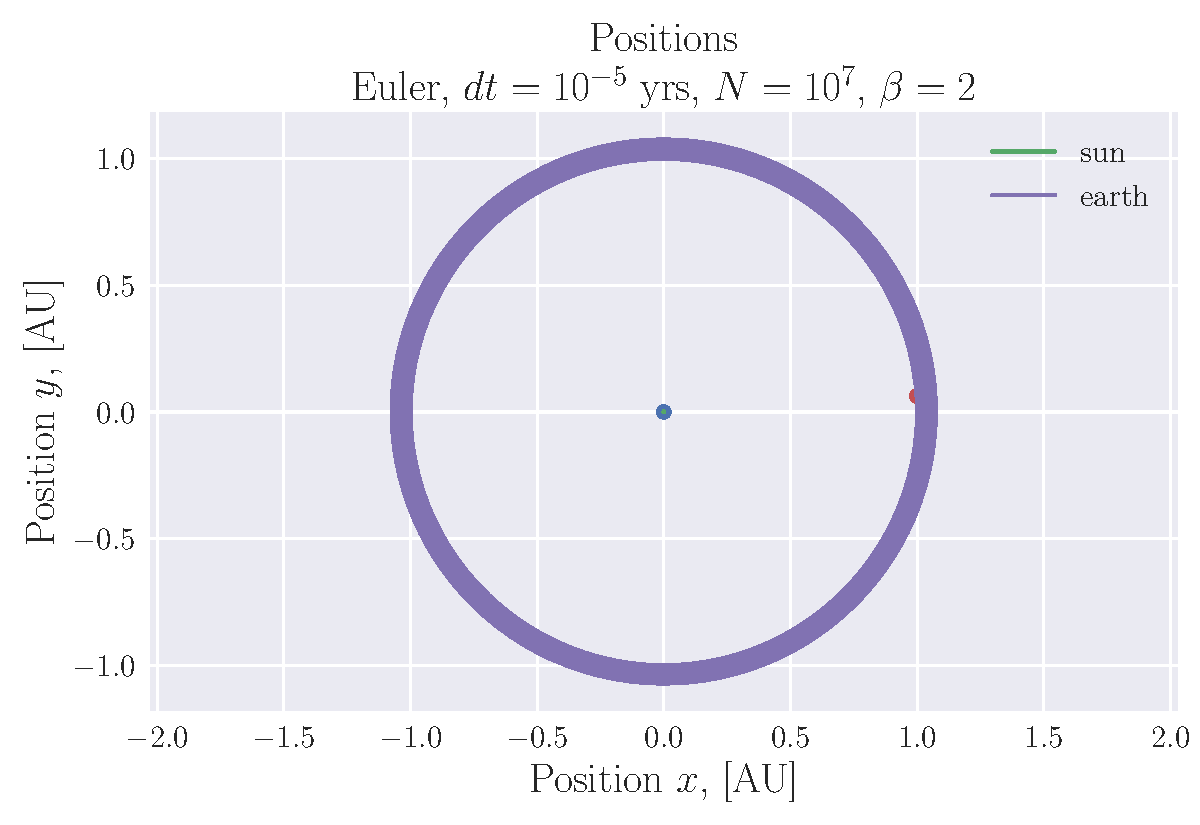
\includegraphics[width=\linewidth]{../output/earth_sun_circ-euler-5-7-2.pdf}
  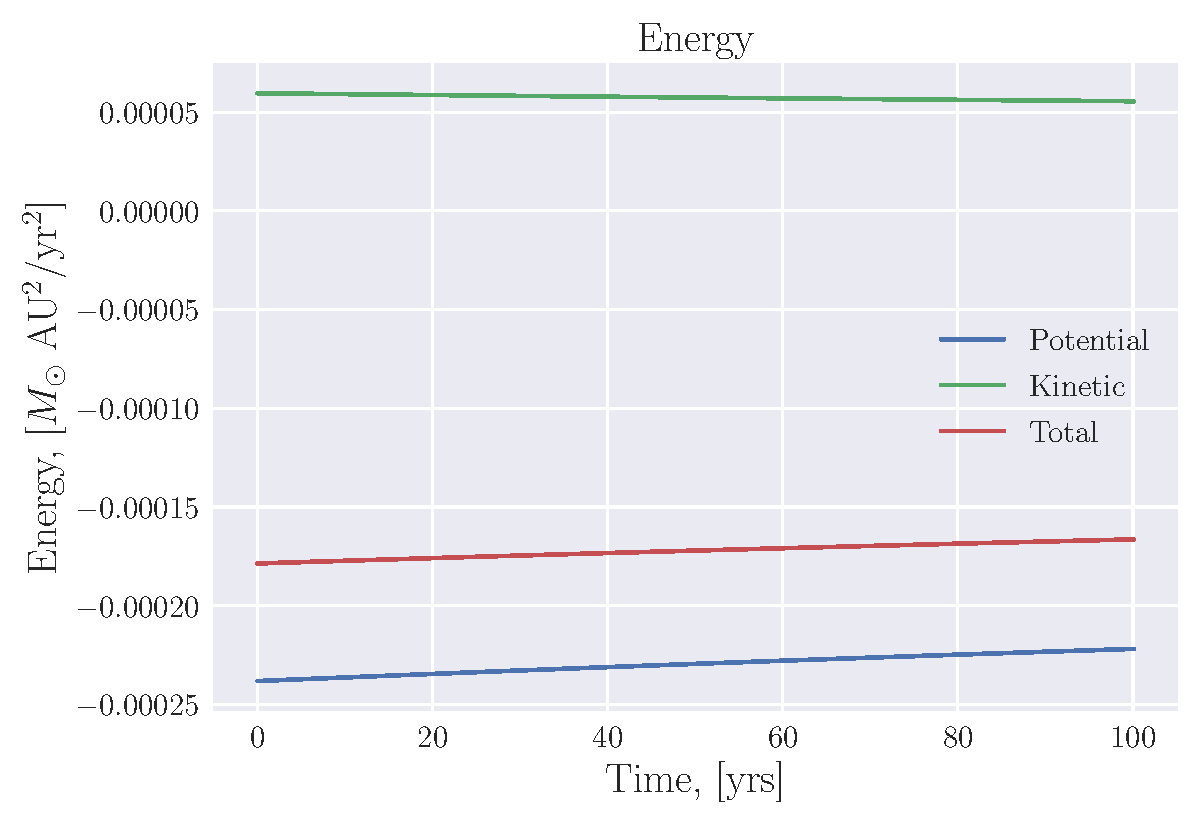
\includegraphics[width=\linewidth]{../output/earth_sun_circ-euler-5-7-2_energy.pdf}
  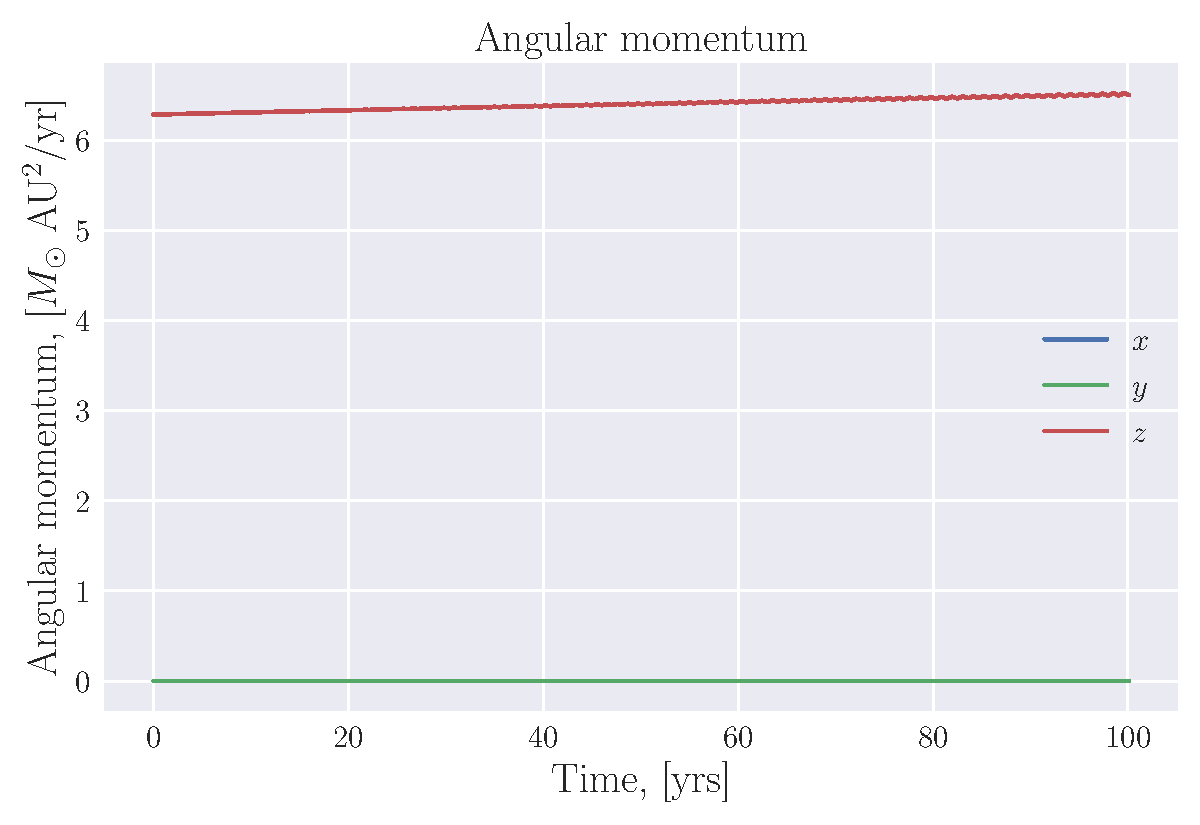
\includegraphics[width=\linewidth]{../output/earth_sun_circ-euler-5-7-2_ang_mom.pdf}
  \caption{The Earth-Sun system with initial conditions that should result in a circular orbit of the Earth around the sun. The simulation is run with a time step of $10^{-5}$ using the normal inverse square law of gravity and the Forward Euler algorithm.}
  \label{fig:earth_sun_circ_euler_dt=5}
\end{figure}

\begin{figure}
  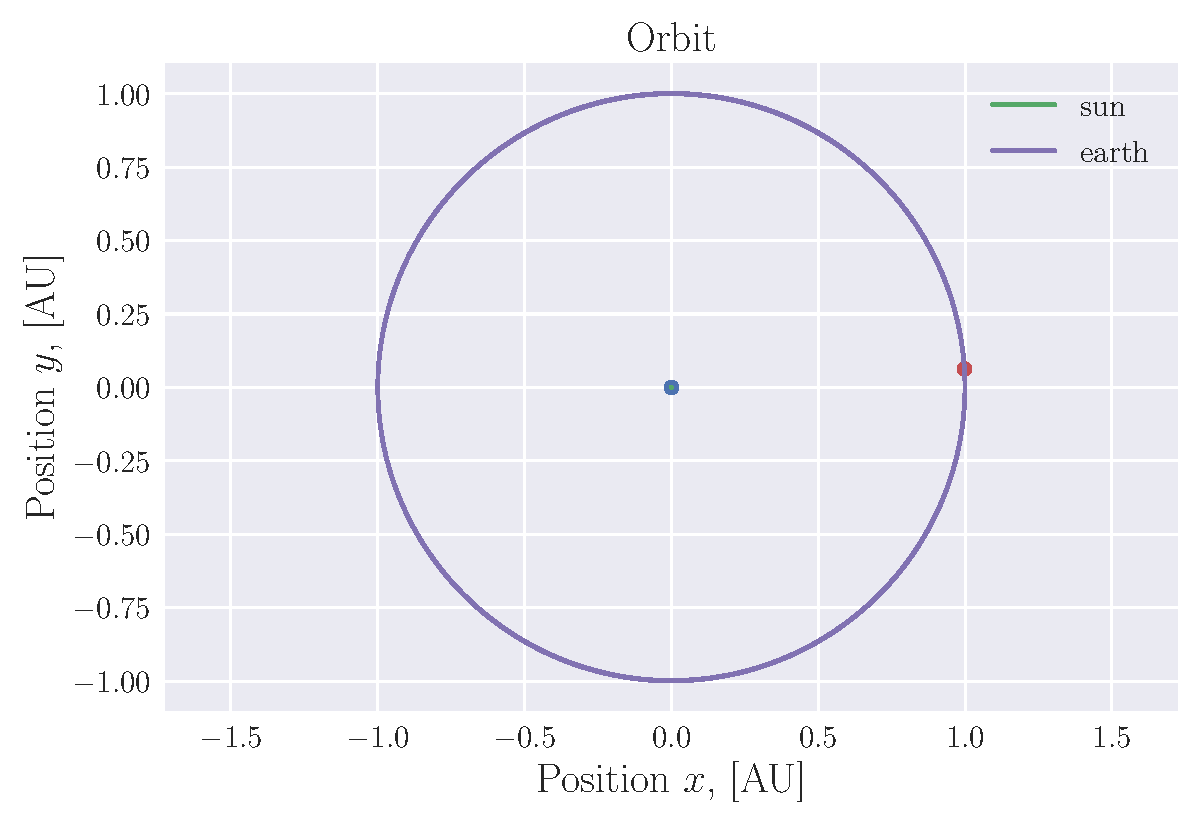
\includegraphics[width=\linewidth]{../output/earth_sun_circ-verlet-5-7-2.pdf}
  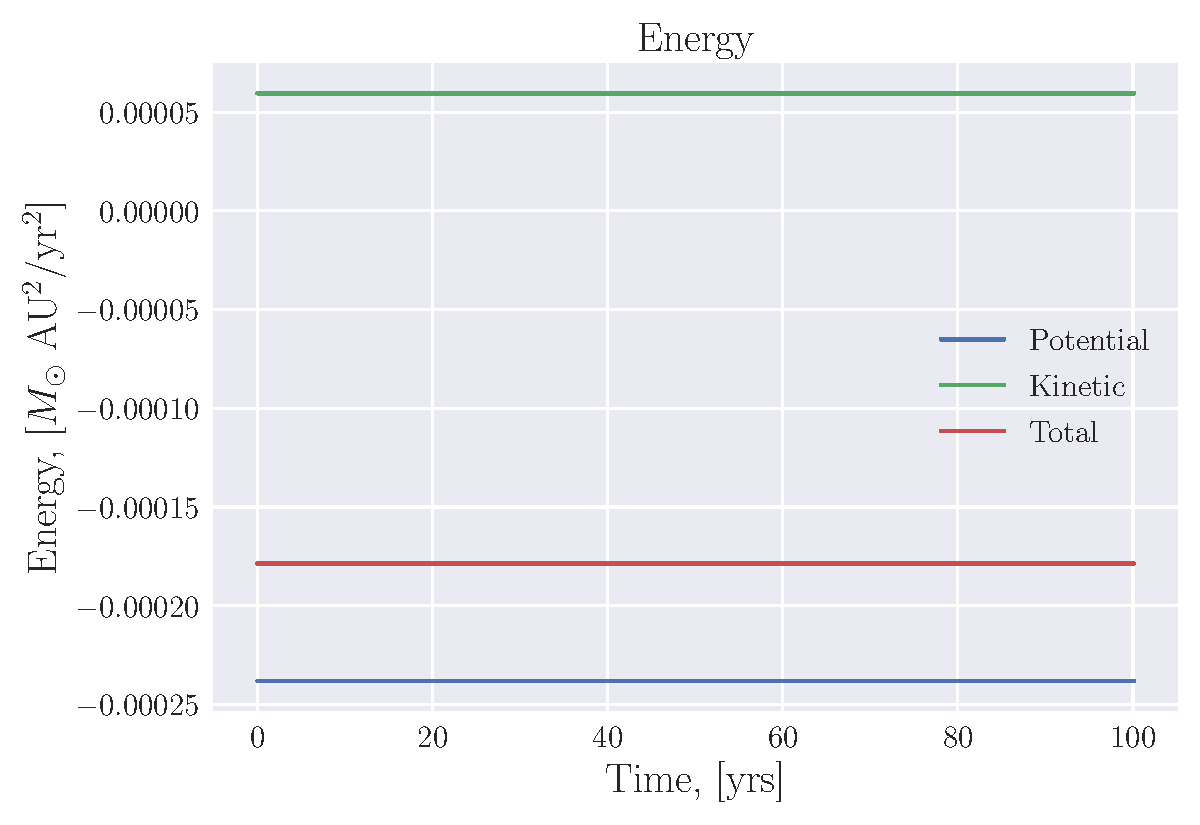
\includegraphics[width=\linewidth]{../output/earth_sun_circ-verlet-5-7-2_energy.pdf}
  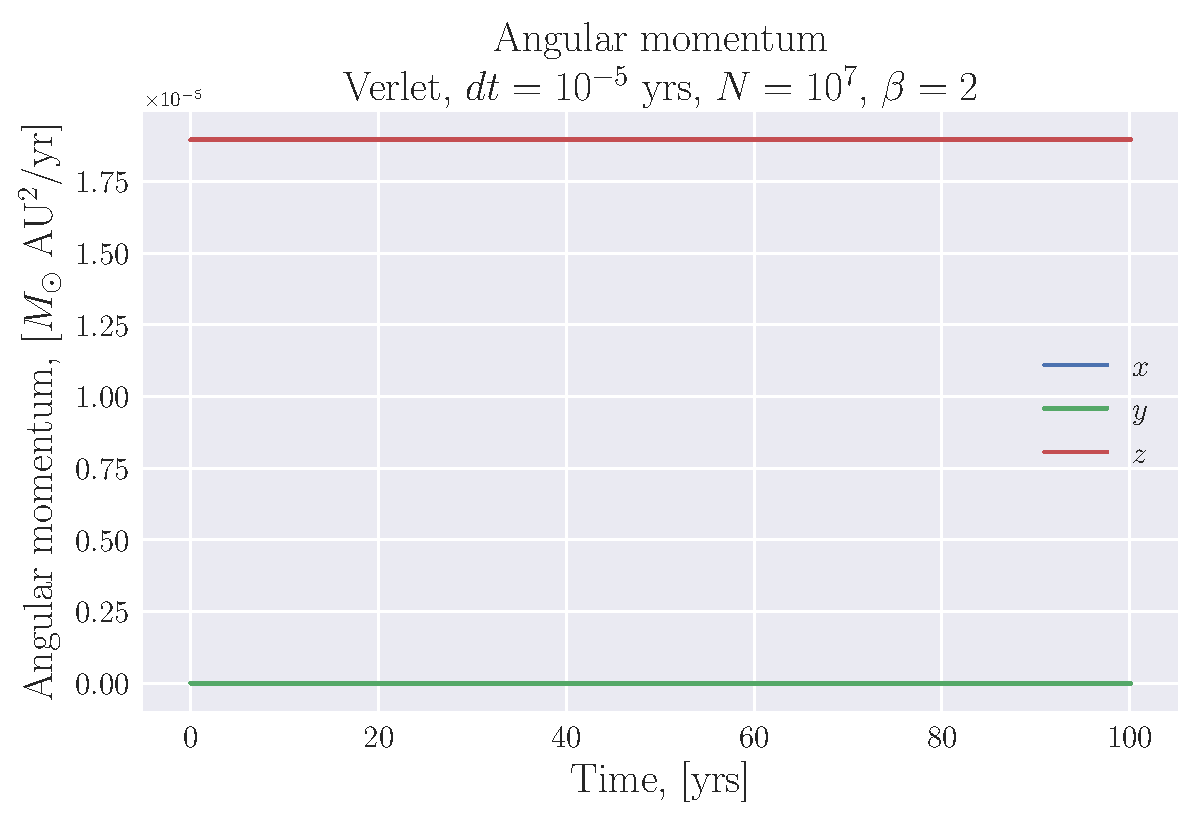
\includegraphics[width=\linewidth]{../output/earth_sun_circ-verlet-5-7-2_ang_mom.pdf}
  \caption{The Earth-Sun system with initial conditions that should result in a circular orbit of the Earth around the sun. The simulation is run with a time step of $10^{-5}$ using the normal inverse square law of gravity and the Velocity Verlet algorithm.}
  \label{fig:earth_sun_circ_verlet}
\end{figure}

\begin{figure}
  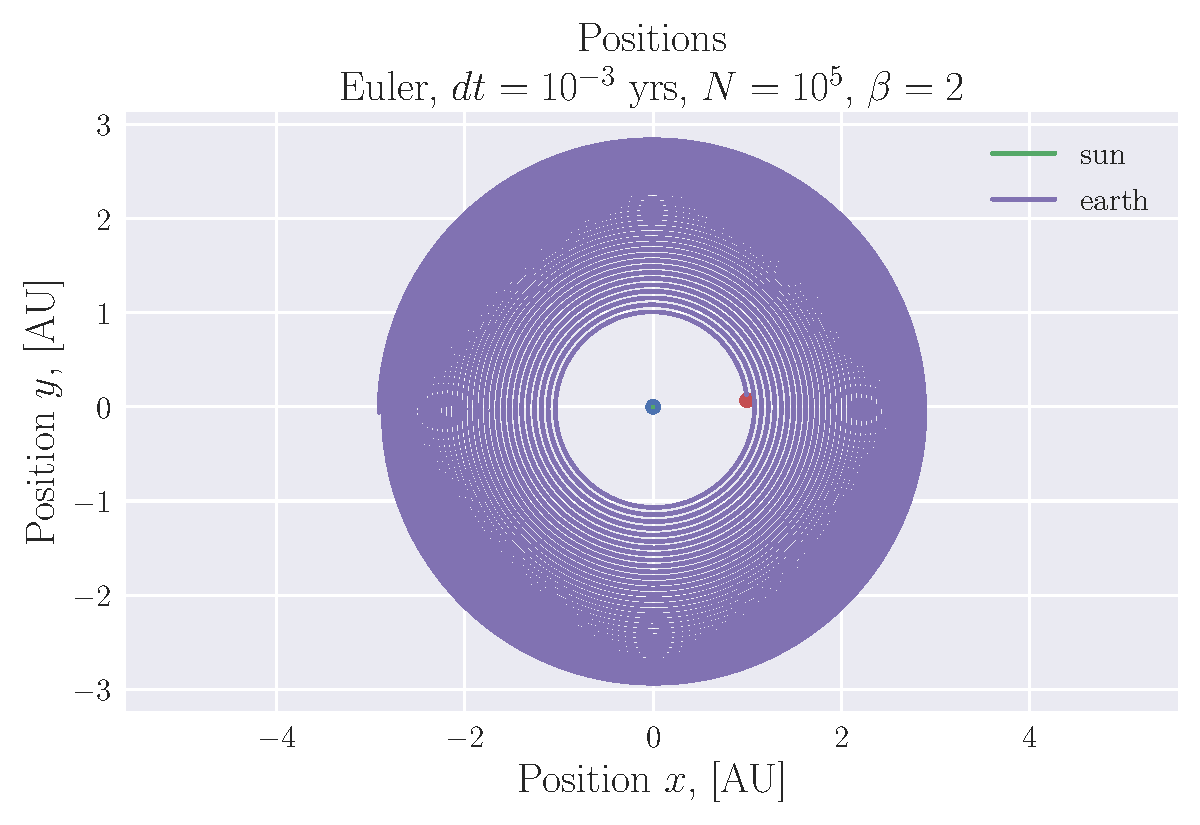
\includegraphics[width=\linewidth]{../output/earth_sun_circ-euler-3-5-2.pdf}
  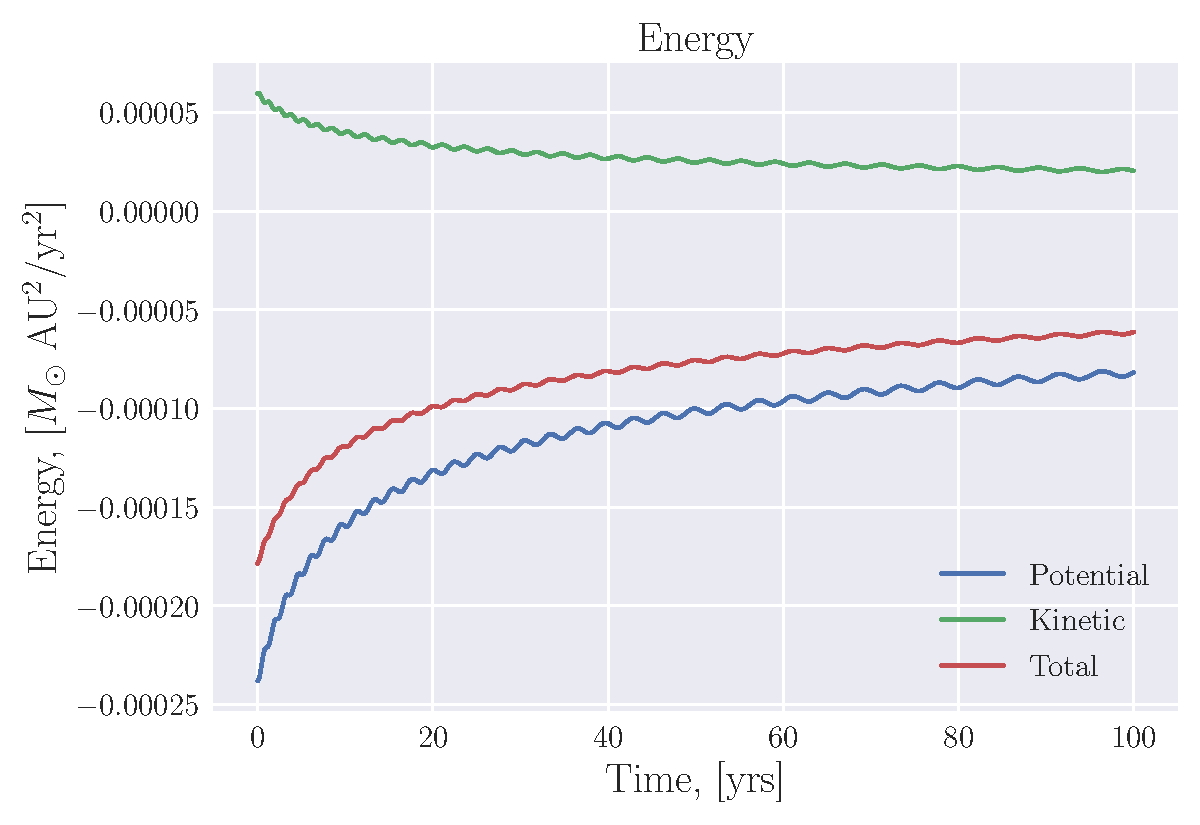
\includegraphics[width=\linewidth]{../output/earth_sun_circ-euler-3-5-2_energy.pdf}
  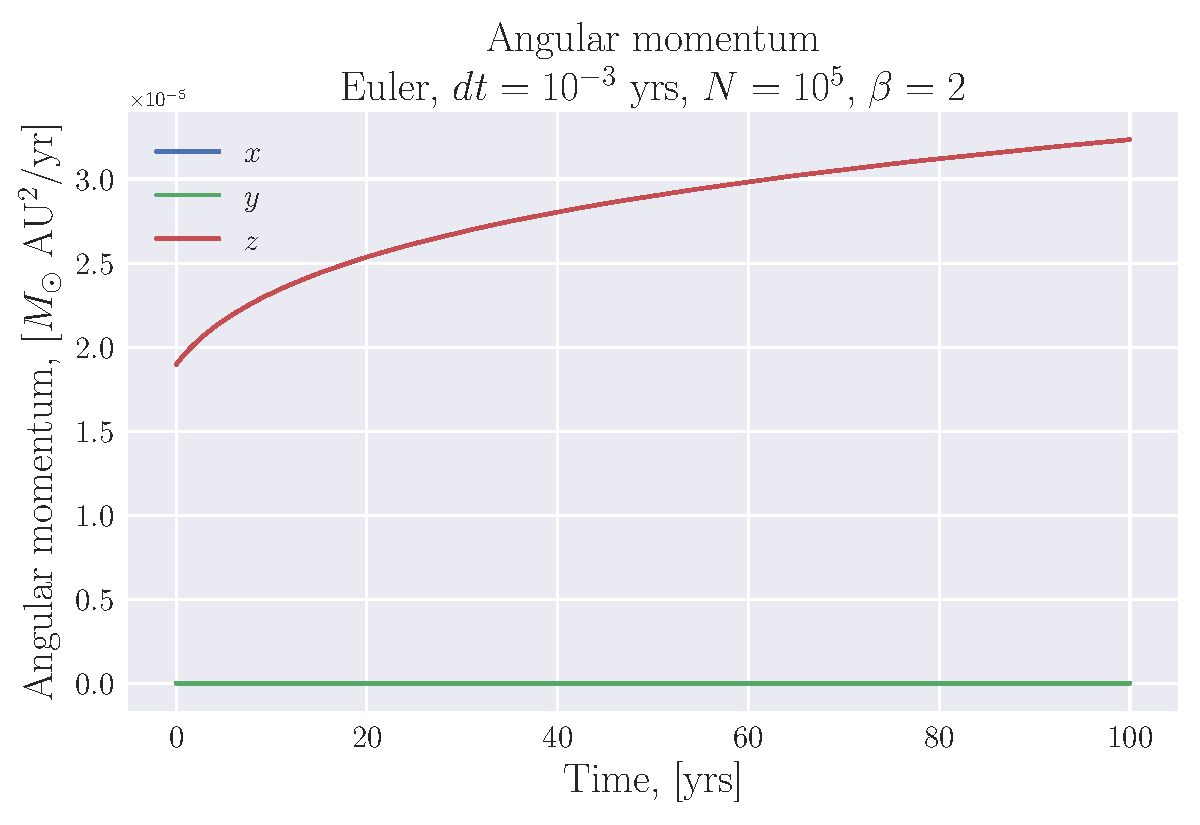
\includegraphics[width=\linewidth]{../output/earth_sun_circ-euler-3-5-2_ang_mom.pdf}
  \caption{The Earth-Sun system with initial conditions that should result in a circular orbit of the Earth around the sun. The simulation is run with a time step of $10^{-3}$ using the normal inverse square law of gravity and the Forward Euler algorithm.}
  \label{fig:earth_sun_circ_euler_dt=3}
\end{figure}


\subsection{Different forms of gravitational force}

Figures \ref{fig:earth_sun_circ_beta=2_75} and \ref{fig:earth_sun_circ_beta=3} show the Earth-Sun system with initial conditions that should produce circular orbits with the inverse square law of gravity. The parameter $\beta$ is set to 2.75 and 3 respectively in the two figures. We do not include the other values of $\beta$ because they are indistinguishable from $\beta = 2.75$. In figure \ref{fig:earth_sun_circ_beta=2_75} it is difficult to see what is happening. Looking at the energy plot, it seems that the planet is spiraling in and out. Opening the data in Ovito, we can see that it is in fact spiraling in and out.

\begin{figure}[h]
	\centering
	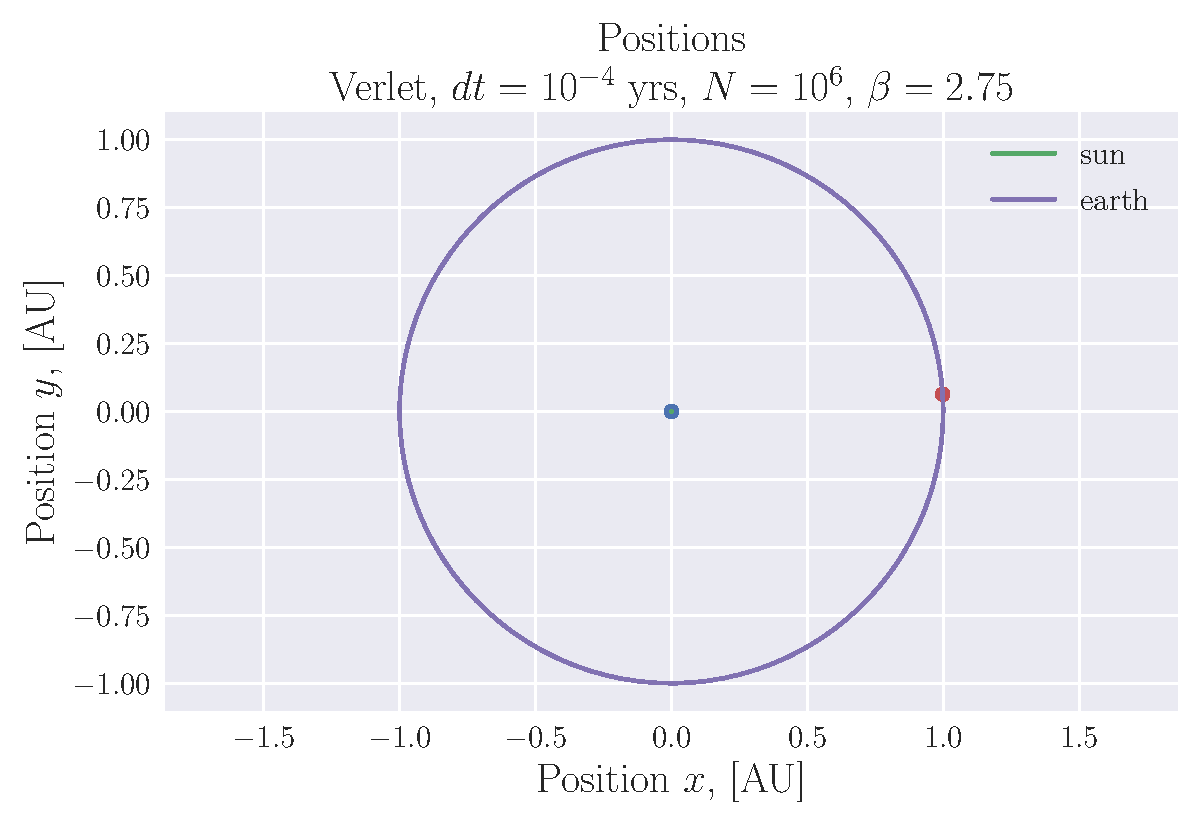
\includegraphics[width=\linewidth]{../output/earth_sun_circ-verlet-4-6-2_75.pdf}
  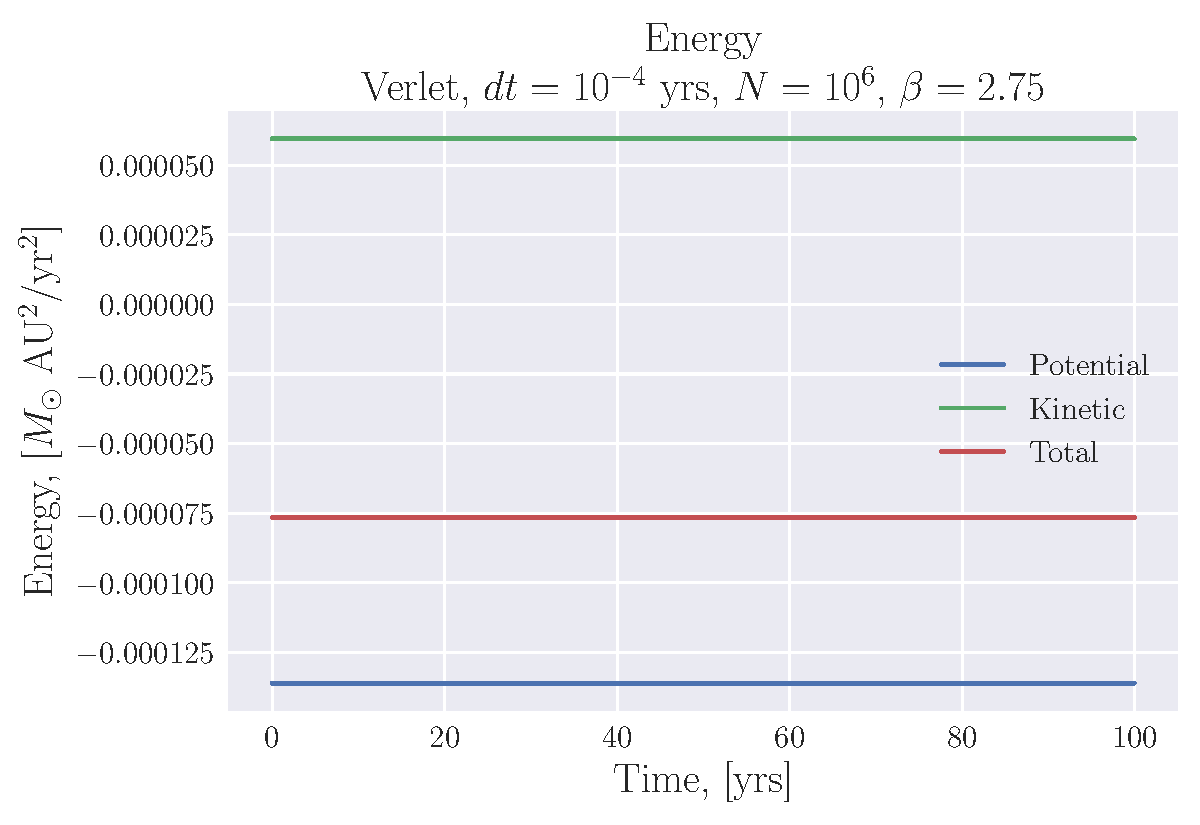
\includegraphics[width=\linewidth]{../output/earth_sun_circ-verlet-4-6-2_75_energy.pdf}
  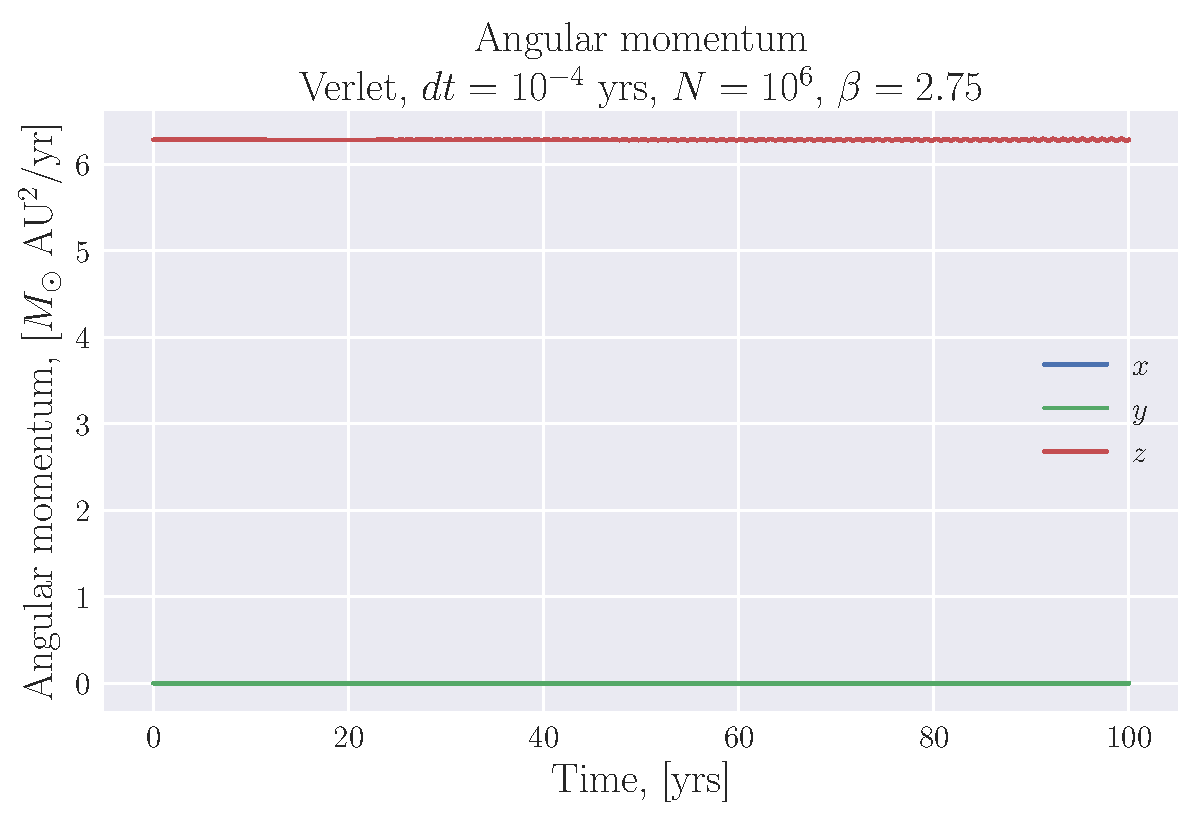
\includegraphics[width=\linewidth]{../output/earth_sun_circ-verlet-4-6-2_75_ang_mom.pdf}
	\caption{In this figure we see orbits, energy and angular momentum of the Earth-Sun system with initial conditions that would produce a circular orbit with the normal inverse square law of gravity. The parameter $\beta = 2.75$.}
	\label{fig:earth_sun_circ_beta=2_75}
\end{figure}

\begin{figure}[h]
	\centering
	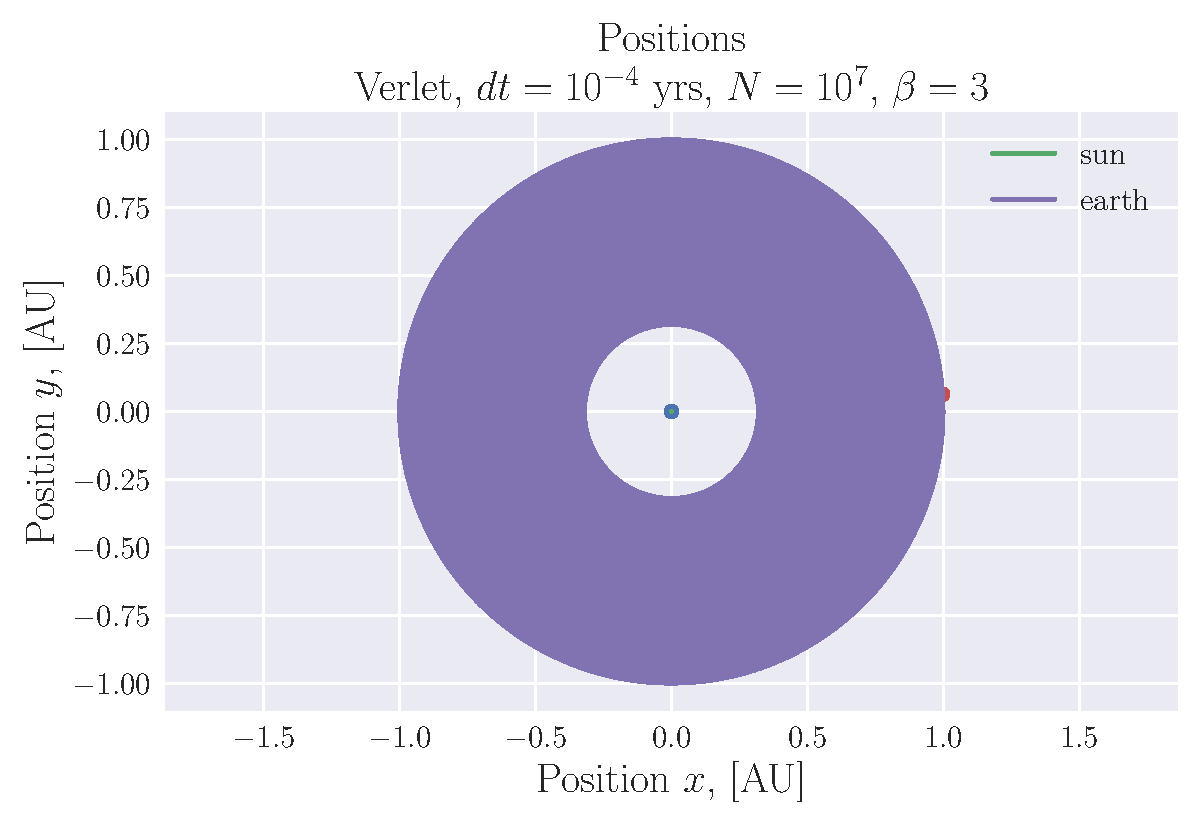
\includegraphics[width=\linewidth]{../output/earth_sun_circ-verlet-4-7-3.pdf}
  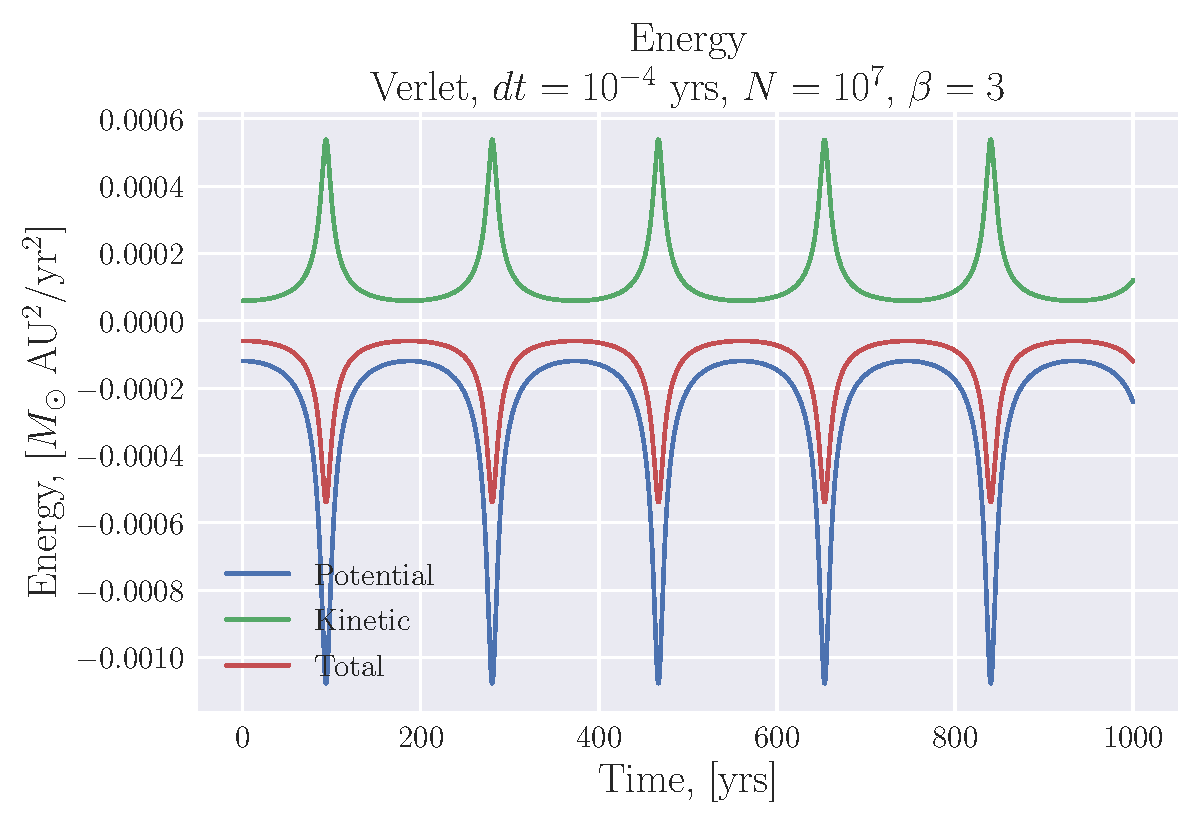
\includegraphics[width=\linewidth]{../output/earth_sun_circ-verlet-4-7-3_energy.pdf}
  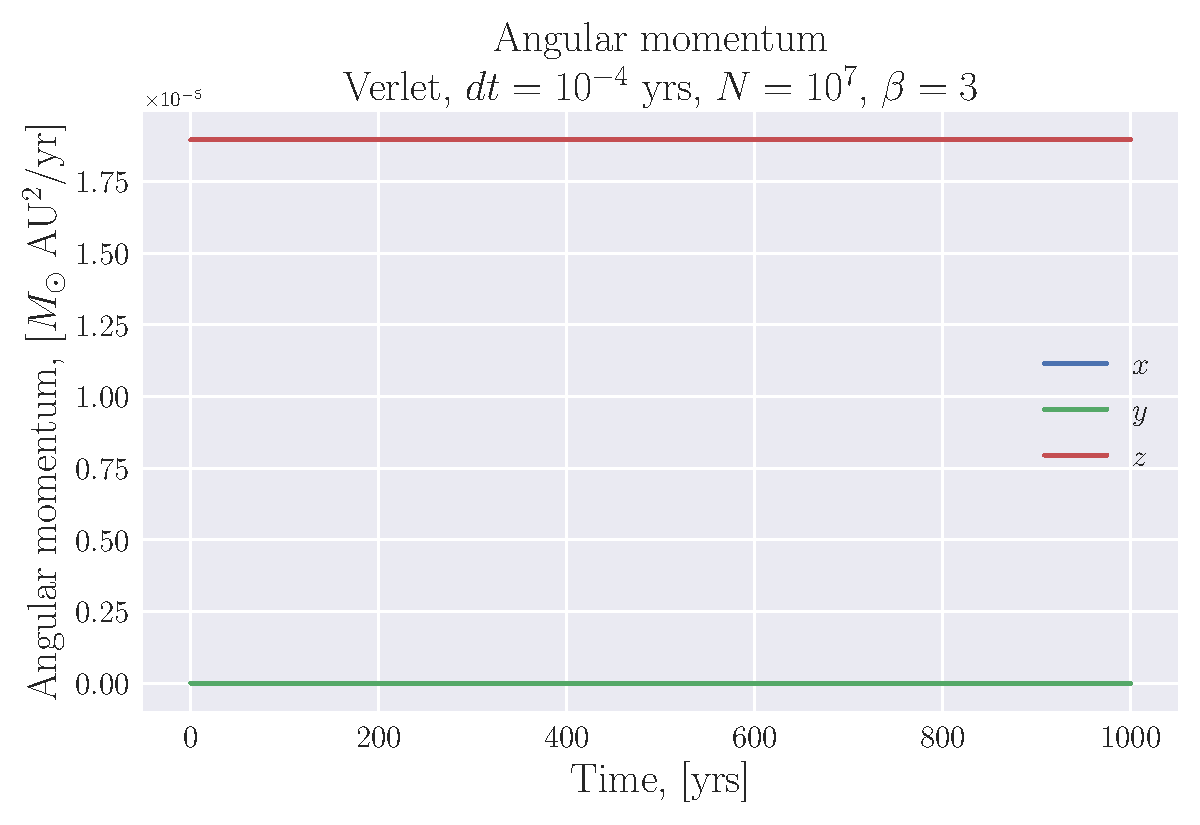
\includegraphics[width=\linewidth]{../output/earth_sun_circ-verlet-4-7-3_ang_mom.pdf}
	\caption{These plots show the orbit, energy and angular momentum of the Earth-Sun system with the parameter $\beta = 3$. The initial conditions are such that the orbit of the Earth around the Sun would be circular with the normal inverse square law of gravity.}
	\label{fig:earth_sun_circ_beta=3}
\end{figure}


\subsection{Escape velocity}

The theoretical escape velocity is known to be $V_{\text{theo}} = 2\pi\sqrt{2} \approx 8.89$AU/yr (this is from equation \eqref{eq:escape_velocity}). When finding the escape velocity we had to test for different tolerances. Lower gave more precise results, however at the cost of computation time. We found that with a tolerance of $\epsilon = 0.001$M$_\odot$AU$^2$/yr$^2$ we got a escape velocity of $v_{\text{esc}} = 8.89$AU/yr, which corresponds to the theoretical value. Time step during simulation was set to $10^{-4}$yr.


\subsection{Many-body problem}

Figures \ref{fig:three_body}, \ref{fig:three_body10} and \ref{fig:three_body1000} shows the orbits of Earth, Jupiter (with ordinary, ten times and thousand times the mass) and the sun. Also we plot the total kinetic and potential energy and the angular momentum of the systems.

\begin{figure}[h]
	\centering
	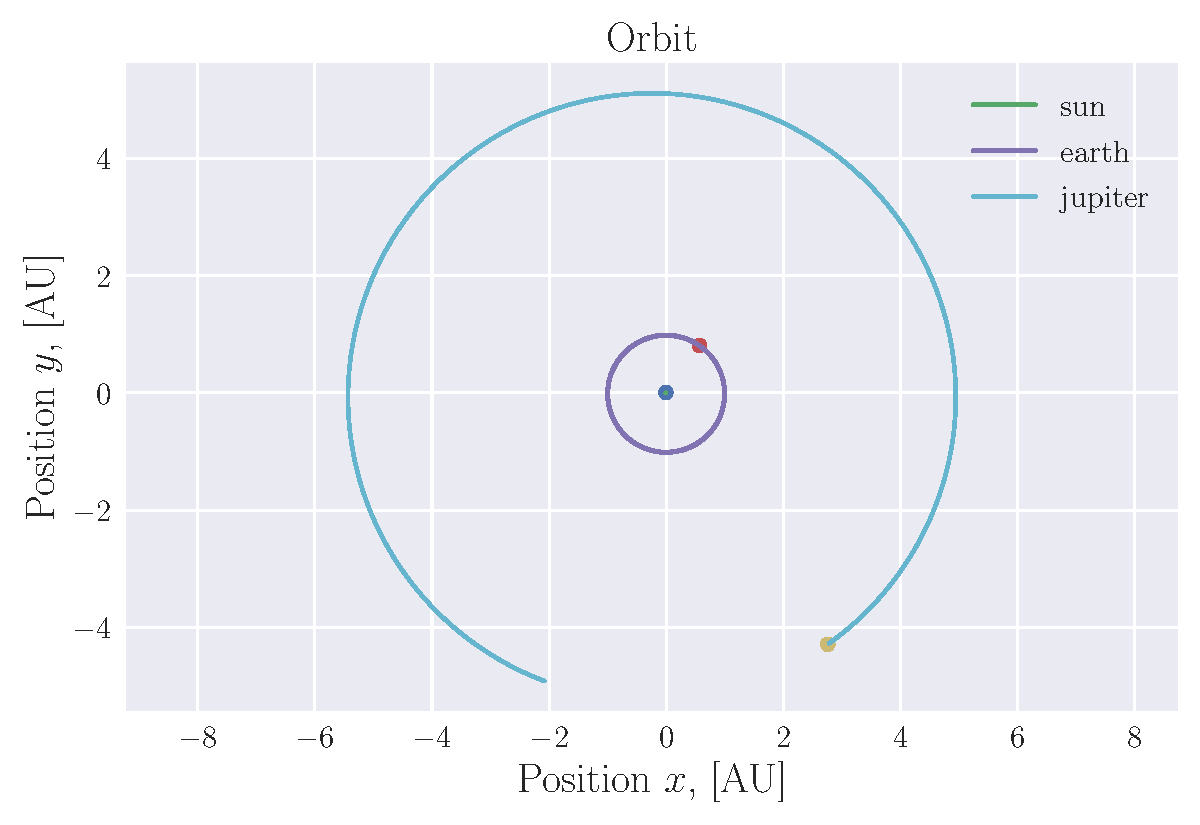
\includegraphics[width=\linewidth]{../output/three_body-verlet-5-6-2.pdf}
	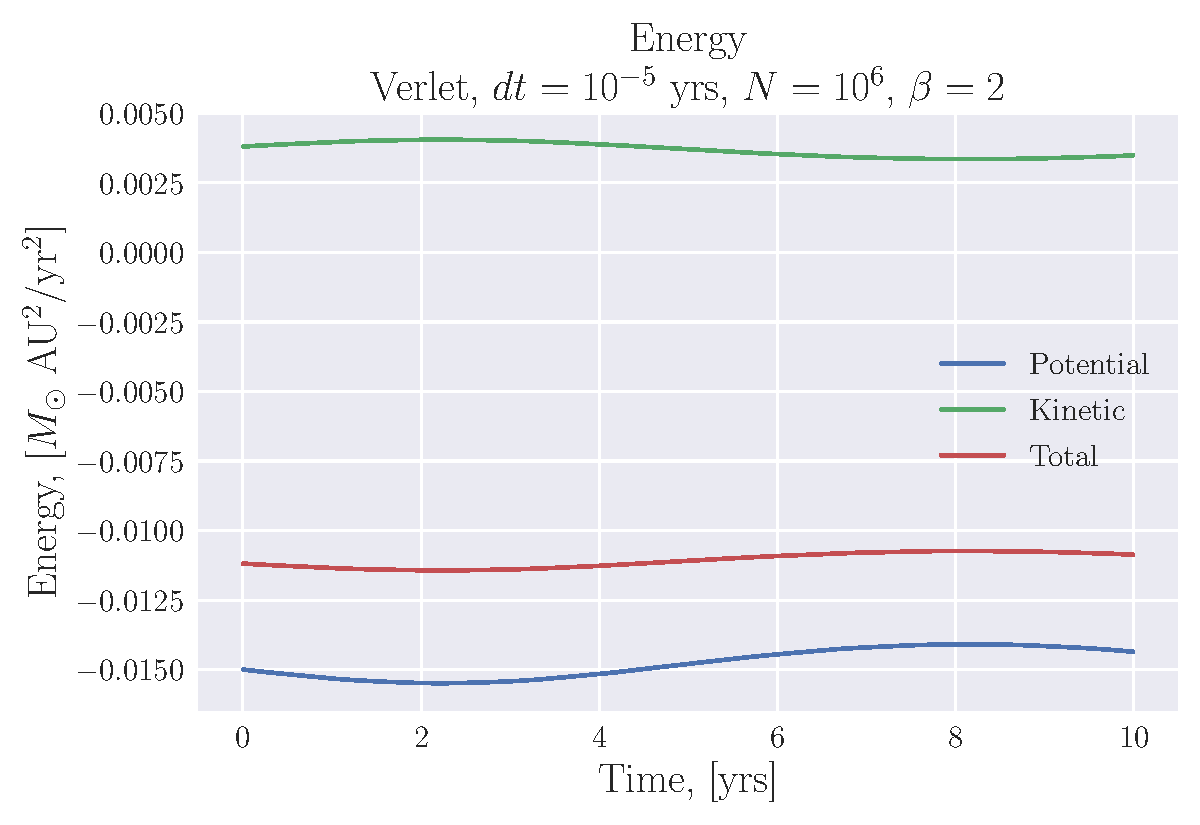
\includegraphics[width=\linewidth]{../output/three_body-verlet-5-6-2_energy.pdf}
	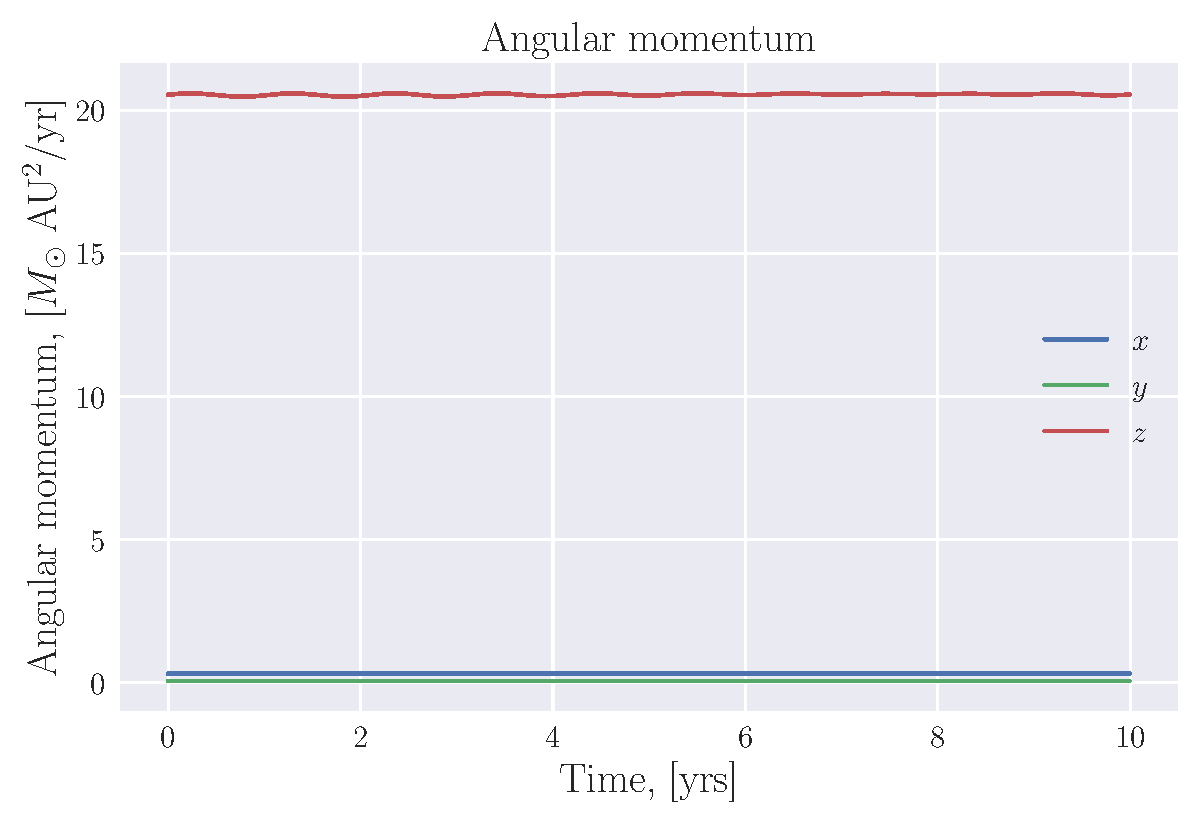
\includegraphics[width=\linewidth]{../output/three_body-verlet-5-6-2_ang_mom.pdf}
	\caption{The figures show the orbit, energy and angular momentum of the Earth, Jupiter (with ordinary mass) and Sun system.}
	\label{fig:three_body}
\end{figure}

\begin{figure}[h]
	\centering
	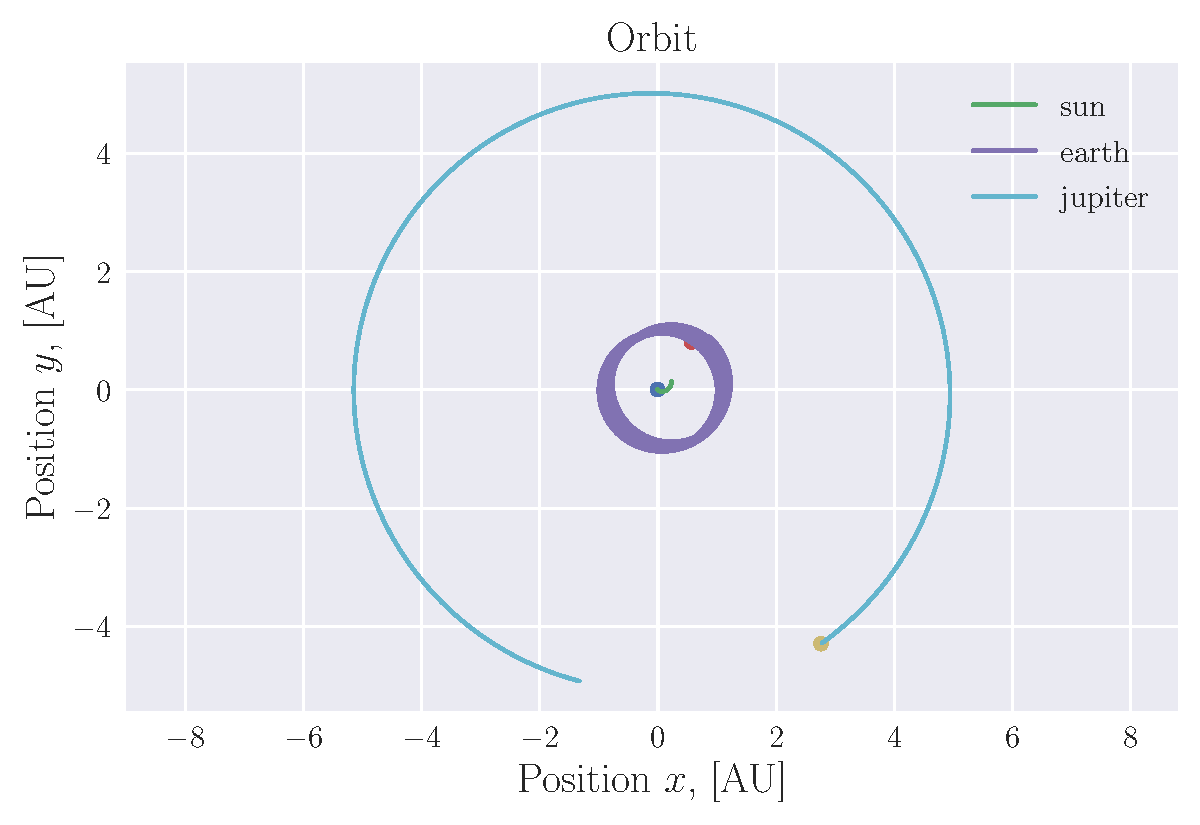
\includegraphics[width=\linewidth]{../output/three_body10-verlet-5-6-2.pdf}
	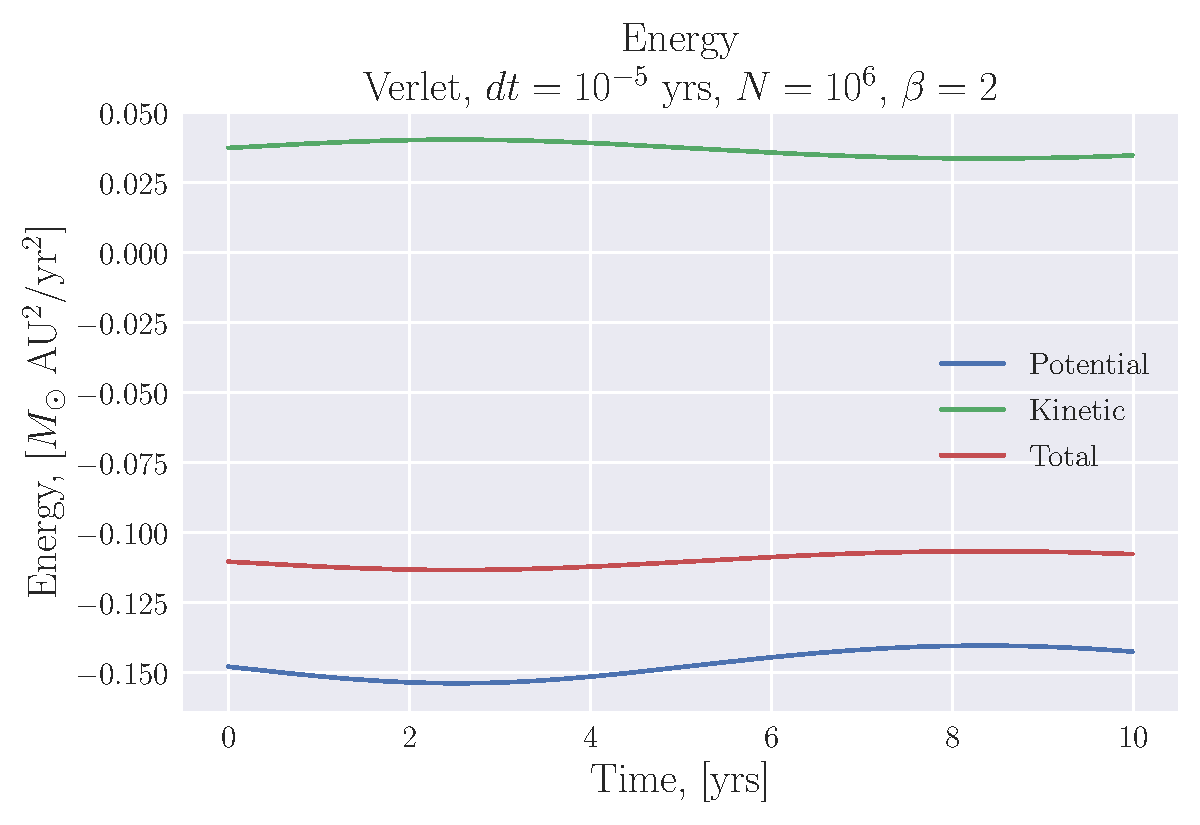
\includegraphics[width=\linewidth]{../output/three_body10-verlet-5-6-2_energy.pdf}
	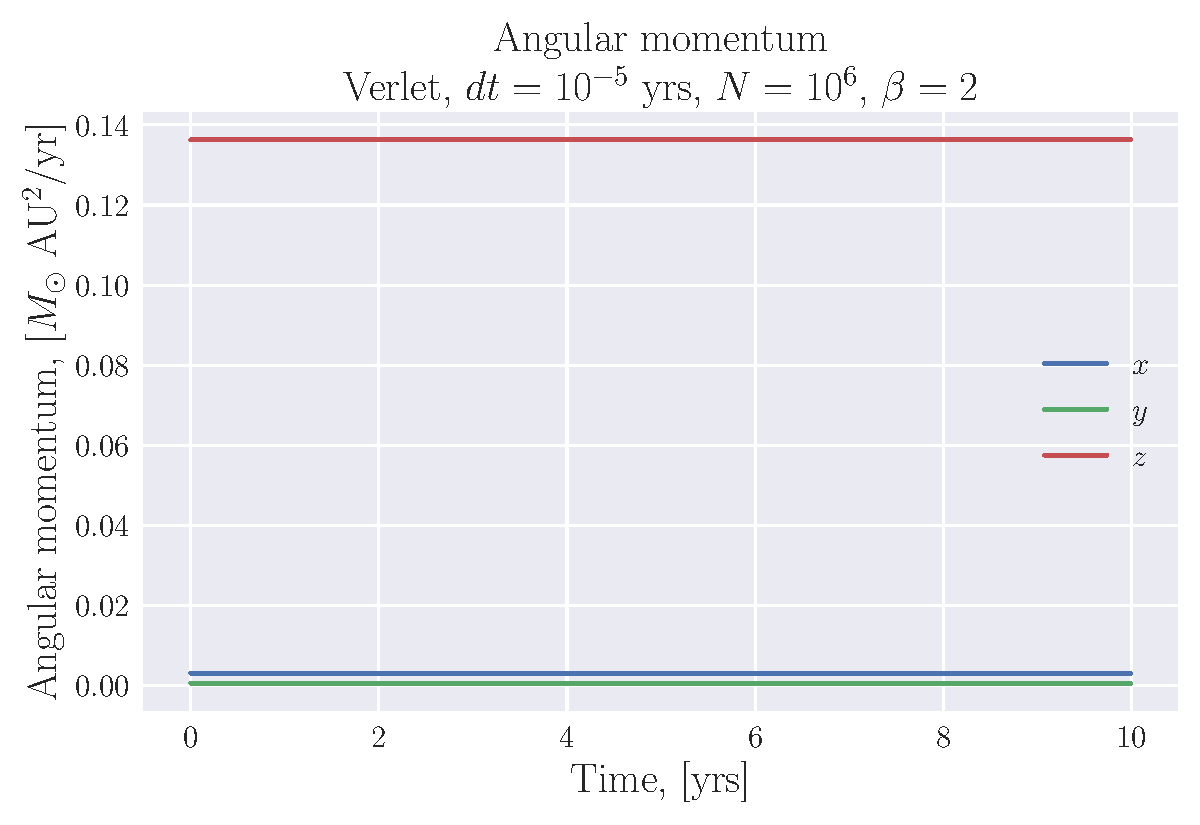
\includegraphics[width=\linewidth]{../output/three_body10-verlet-5-6-2_ang_mom.pdf}
	\caption{The figures show the orbit, energy and angular momentum of the Earth, Jupiter (with ordinary mass) and Sun system. Here we have multiplied Jupiter's mass with 10.}
	\label{fig:three_body10}
\end{figure}

\begin{figure}[h]
	\centering
	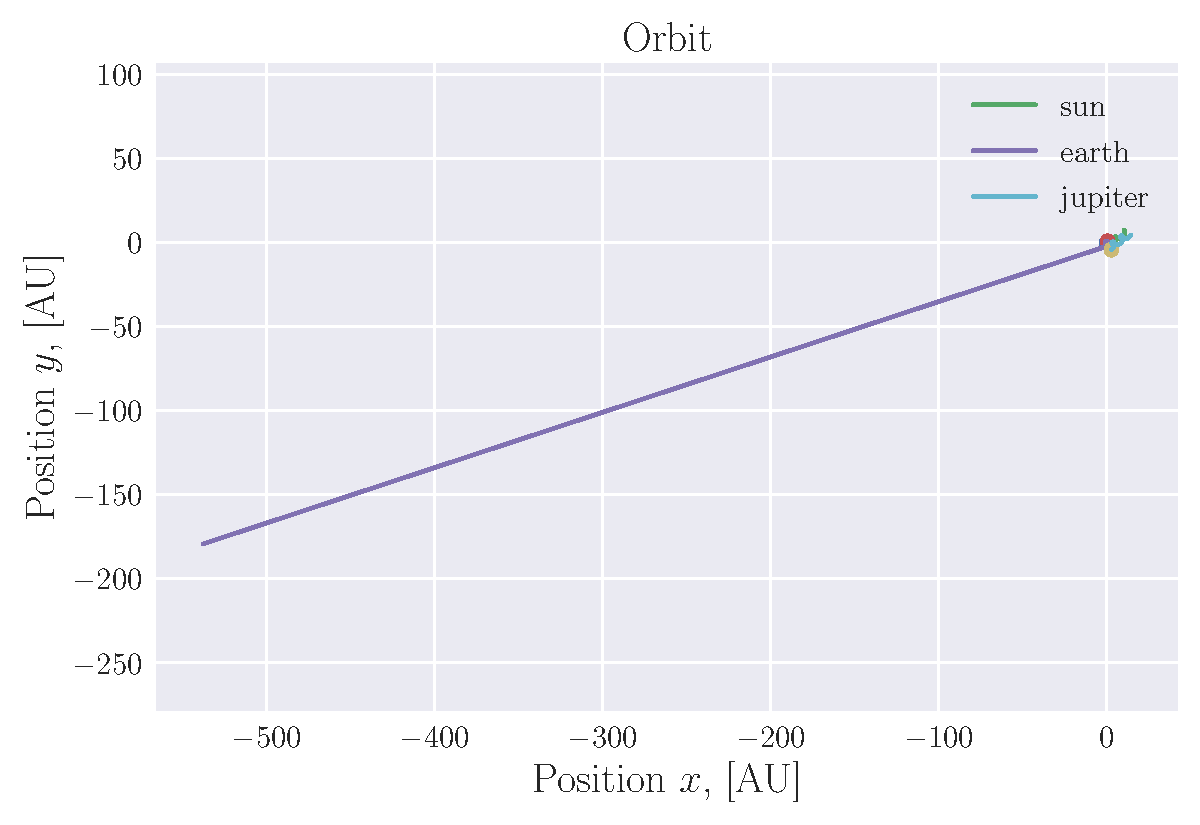
\includegraphics[width=\linewidth]{../output/three_body1000-verlet-5-6-2.pdf}
	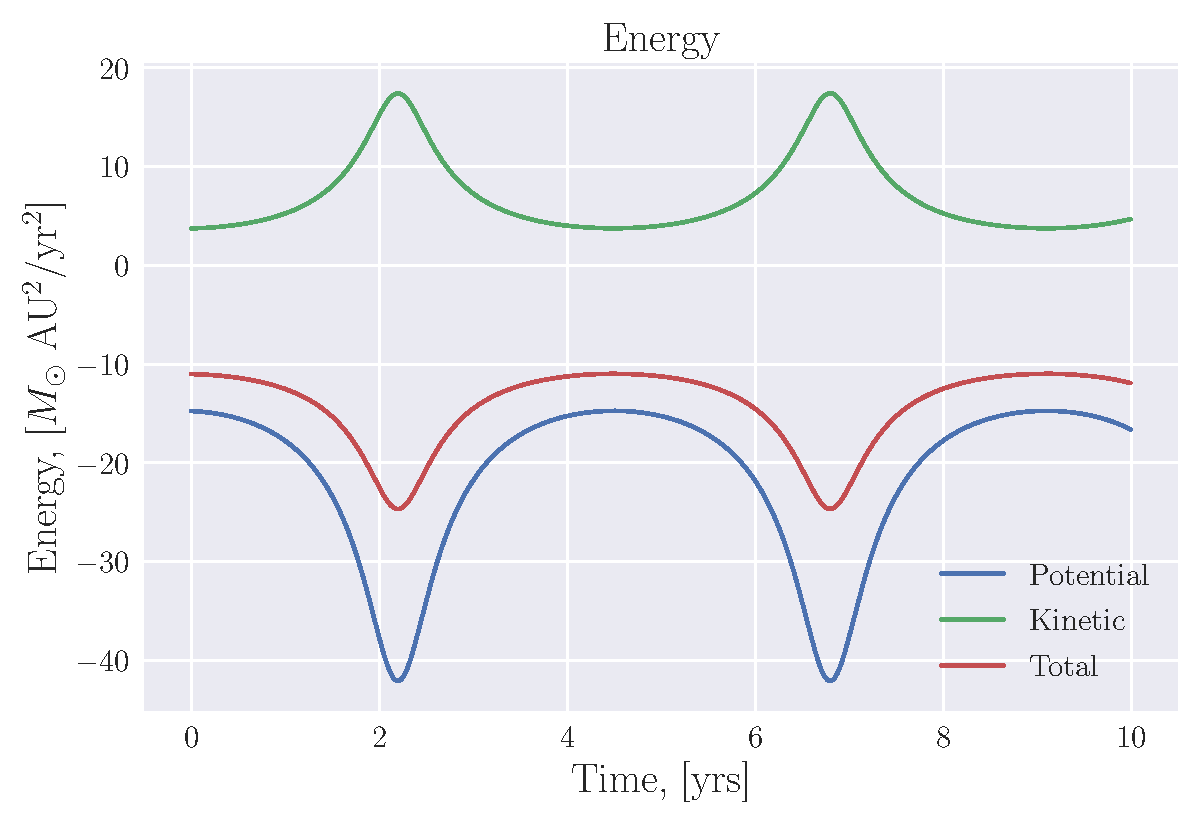
\includegraphics[width=\linewidth]{../output/three_body1000-verlet-5-6-2_energy.pdf}
	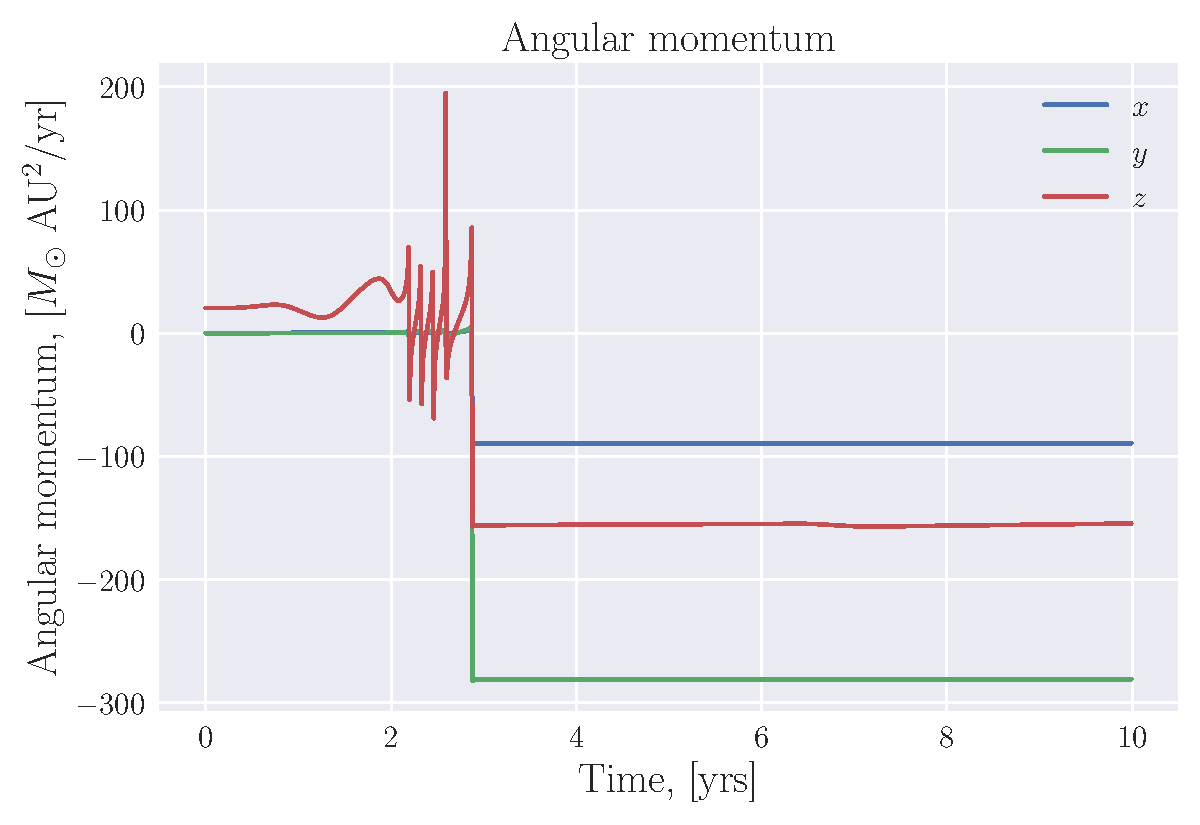
\includegraphics[width=\linewidth]{../output/three_body1000-verlet-5-6-2_ang_mom.pdf}
	\caption{The figures show the orbit, energy and angular momentum of the Earth, Jupiter and Sun system. Here we have multiplied Jupiter's mass with $10^3$.}
	\label{fig:three_body1000}
\end{figure}
Figure \ref{fig:all} shows the orbits of all the bodies during a full simulation of the Solar System, as well as the total kinetic and potential energy and the angular momentum of the system.

\begin{figure}[h]
	\centering
	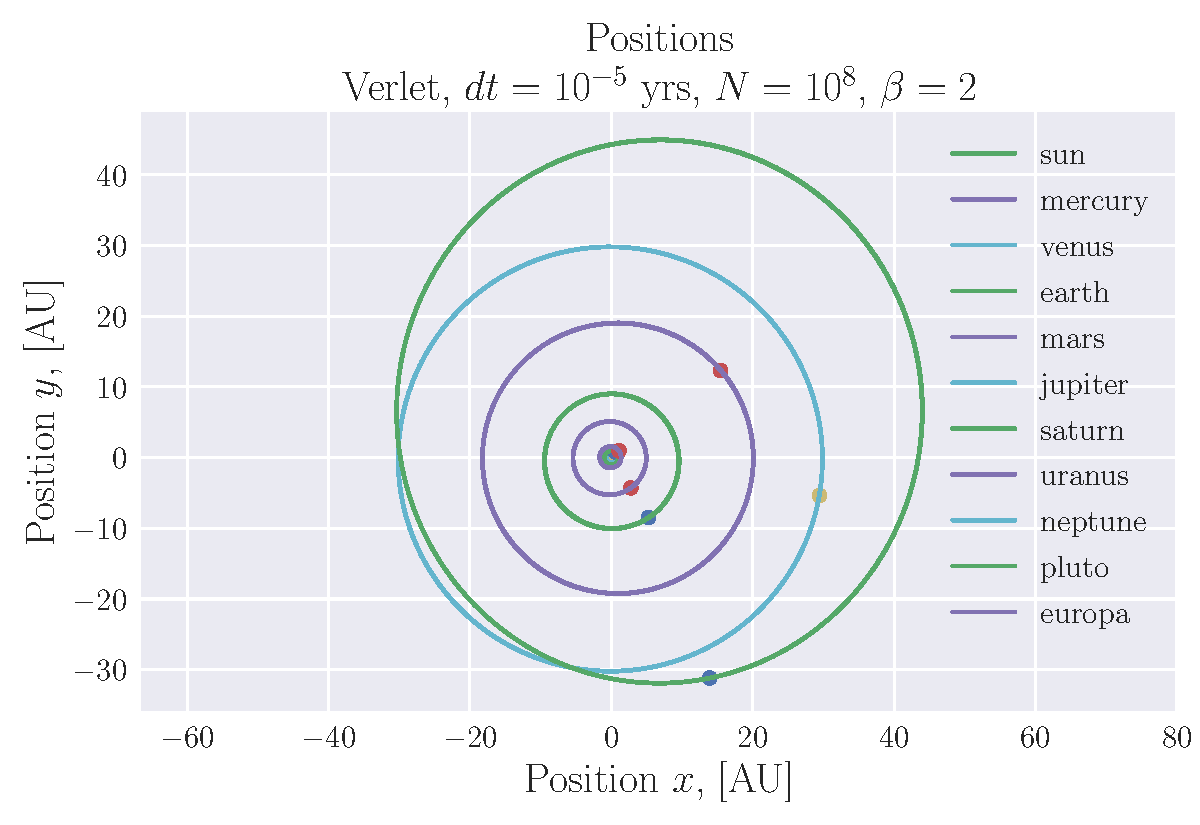
\includegraphics[width=\linewidth]{../output/all-verlet-5-8-2.pdf}
  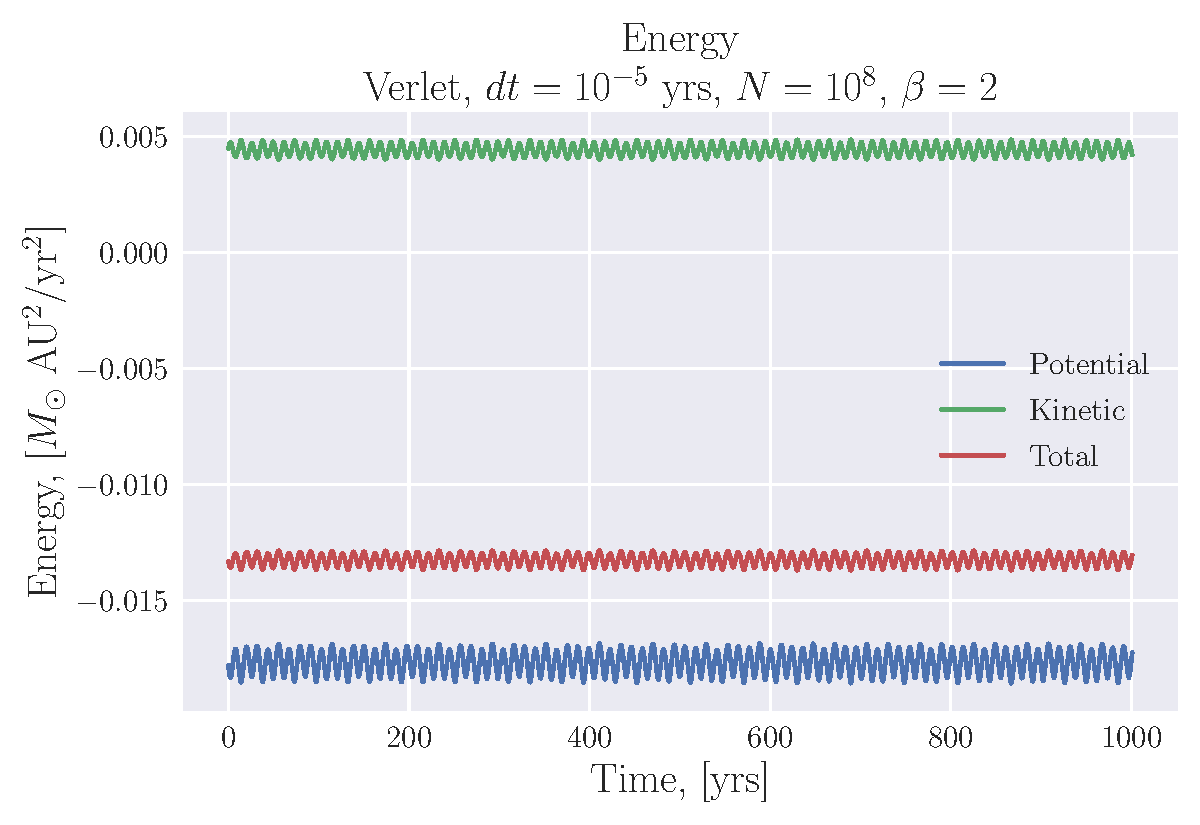
\includegraphics[width=\linewidth]{../output/all-verlet-5-8-2_energy.pdf}
  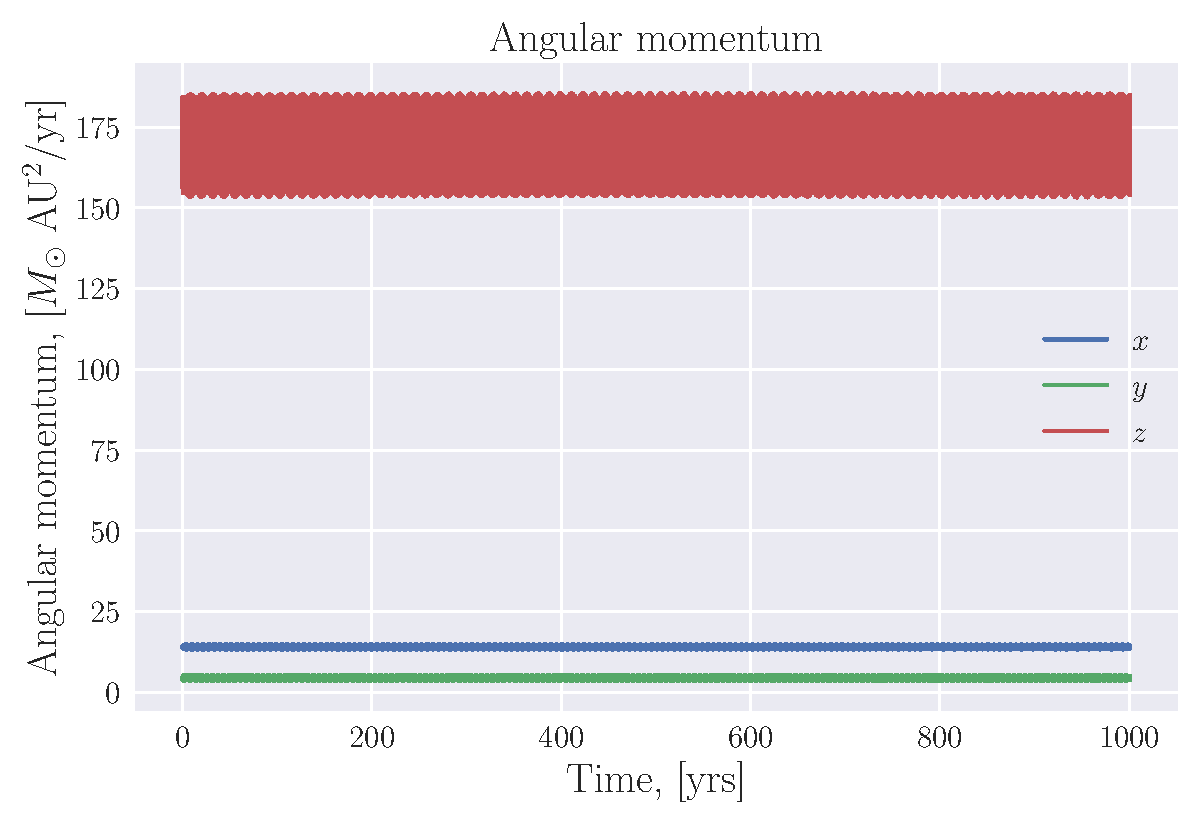
\includegraphics[width=\linewidth]{../output/all-verlet-5-8-2_ang_mom.pdf}
	\caption{In these figures we see the orbits, energy and angular momentum of all the bodies in a full-blown simulation of the Solar System. Included are the Sun, all the planets (including Pluto) and Europa (one of the moons of Jupiter).}
	\label{fig:all}
\end{figure}


\subsection{General relativity}

We ended up doing the tests for three different time steps (see \ref{tab:general_relativity}). Notice that with a time step of around 3.16 seconds, we got a precession of 43.26$''$ which is quite close to the theoretical value of 43$''$. Time step of 31.56 seconds was also quite close, with a value of 40.43$''$. Our first result however, showed precession in the opposite direction.
\begin{table}[h]
	\begin{tabular}{|l|l|l|}
		\hline
		Timestep {[}s{]} & Integration points N & Result {[}arcseconds{]} \\
		\hline
		315.56              & $10^7$          & -0.79               \\
		31.56               & $10^8$          & 40.43                 \\
		3.16                & $10^9$          & 43.26	\\
		\hline
	\end{tabular}
	\caption{In this table you have the different time steps we tested for, in units of seconds. The second column shows the number of integration points needed, and the last column is our results in arcseconds.
	\label{tab:general_relativity}}
\end{table}
\\
We wanted to test for smaller time steps, however we exceeded the maximum array-length. Also, because our last result were quite close to the theoretical, we opted against it.



\section{Discussion}

testing and comparing algorithms(discuss eventual differences between the verlet algorithm and the euler algorithm. Consider also the numver of flops involved and perform a timing of the two algorithm for equal final times.)

The different forms of the gravitational force proved to result in very different behaviour of the Earth-Sun system.

As we mentioned, when calculating the escape velocity, we cannot be infinitely precise. There is a constant trade-off between precision and computation time. We don't believe our method and calculations are wrong, as we are studying a very simple system. What we do acknowledge however, is that we could get a more precise answer.

% Many body
We simulated several many-body situations, namely the Earth, Jupiter and Sun (where Jupiter has different masses), and the entire solar system. When Simulating different masses of Jupiter we got quite different results. The real-world mass of Jupiter clearly affected the orbits of both the Earth and the Sun, but

When including a general relativistic correction, we ended up at the observed value. However it is worth discussing the fact that we only arrived at the right answer for one time step, namely 3.16 seconds. Ideally we would want to test for lower time steps, to confirm that this was not a fluke. However, seeing that we arrived very close for the time step 31.56 seconds, it seems unlikely.



\section{Conclusion}

For some of the systems, the results step size were very different with different step sizes. 




\onecolumngrid
\vspace{1cm} % some extra space
\newpage

\begin{thebibliography}{}
\bibitem[]{oppgavetekst} Department of Physics, Univeristy of Oslo, Fall semester 2020, Computational Physics I FYS3150/FYS4150, Project 3.
\bibitem[]{NASA} Ryan S. Park, Alan B. Chamberlin, NASA, 27. October 2020, https://ssd.jpl.nasa.gov/horizons.cgi\#top.

\end{thebibliography}


\end{document}
